% Submission manuscript. Compile with pdfLaTeX (the Overleaf default).
\documentclass[12pt]{article}
\usepackage[a4paper,margin=1in]{geometry}
\usepackage[utf8]{inputenc}
\usepackage[T1]{fontenc}
\usepackage{amsmath}
\usepackage{newtxtext,newtxmath}
\usepackage{microtype}
\usepackage{graphicx}
\usepackage{booktabs}
\usepackage{makecell}
\usepackage{setspace}
\usepackage{newunicodechar}
\usepackage{xcolor}
\usepackage[hidelinks]{hyperref}

\graphicspath{{figures/}}

\newunicodechar{−}{\ensuremath{-}}
\newunicodechar{–}{--}
\newunicodechar{×}{\ensuremath{\times}}
\newunicodechar{≤}{\ensuremath{\leq}}
\newunicodechar{≈}{\ensuremath{\approx}}
\newunicodechar{±}{\ensuremath{\pm}}
\newunicodechar{∈}{\ensuremath{\in}}
\newunicodechar{→}{\ensuremath{\to}}
\newunicodechar{←}{\ensuremath{\leftarrow}}
\newunicodechar{·}{\ensuremath{\cdot}}
\newunicodechar{Σ}{\ensuremath{\Sigma}}
\newunicodechar{π}{\ensuremath{\pi}}
\newunicodechar{μ}{\ensuremath{\mu}}
\newunicodechar{ρ}{\ensuremath{\rho}}
\newunicodechar{τ}{\ensuremath{\tau}}
\newunicodechar{Δ}{\ensuremath{\Delta}}
\newunicodechar{ŷ}{\ensuremath{\hat{y}}}

\begin{document}

\begin{singlespace}
\begin{center}
{\LARGE\bfseries Separating mixing from selection: a leave-one-line-out\\[2pt]
benchmark and an audit protocol for cross-cell-line\\[2pt]
perturbation evaluation}\\[18pt]
{\large Zhenghao Zhu$^{1}$, Di Cui$^{1,*}$}\\[6pt]
{\small $^{1}$Heze University, Heze, Shandong, China}\\[4pt]
{\small $^{*}$Correspondence: cuidi-nano@hotmail.com}\\
{\small Running title: Mixing and selection in cross-line benchmarks}
\end{center}
\end{singlespace}

\section*{Abstract}

Cross-cell-line scores move for several reasons. Prediction quality is one. Target selection, the reference pool, and scoring policy are others. Two leave-one-line-out panels separate them. Four harmonized lines gave 5,486 queries; five heterogeneous lines gave 18,678. Every query has a response row in the held-out line and at least one source. H1 rows are scVI-decoded, not measured. Swapping in a DESeq2 table for 150 H1 targets moved the pooled equal-mix score by less than 0.01; a Hallmark signal survived, per-target agreement did not. We removed the target gene's coordinate and ranked the true response against the full pool (PDS). A training-free equal mix of matched source responses beat the target-agnostic mean in all nine holdouts, by 0.087 to 0.329 PDS. Reweighting and aggregation added less than 0.01. Gene-shuffled truth still scored 0.655. Pool composition moved the equal-mix level from 0.438 to 0.996. Per-target oracle gains were 0.10 to 0.13 in the harmonized tier and 0.06 to 0.11 in the heterogeneous tier; one global rule retained 0.032 to 0.094 and $-$0.005 to +0.021. The oracle gap mixes target heterogeneity with rule-selection optimism. Equal mixing beat a GEARS adaptation by 0.16 to 0.19 PDS in every Tier A fold. With the corrected scorer, 50 to 100 k-means labels helped three harmonized holdouts; at 20 labels, k-means beat random in four of five heterogeneous holdouts. A drug panel grown from seven to twelve lines sat near the PDS ceiling. Mixing, target composition, scoring policy, and label access need separate reporting.

\noindent\textbf{Keywords:} perturbation prediction; cross-cell-line transfer; Perturb-seq; benchmark; retrieval; virtual cell

\section*{Graphical abstract}

\begin{center}
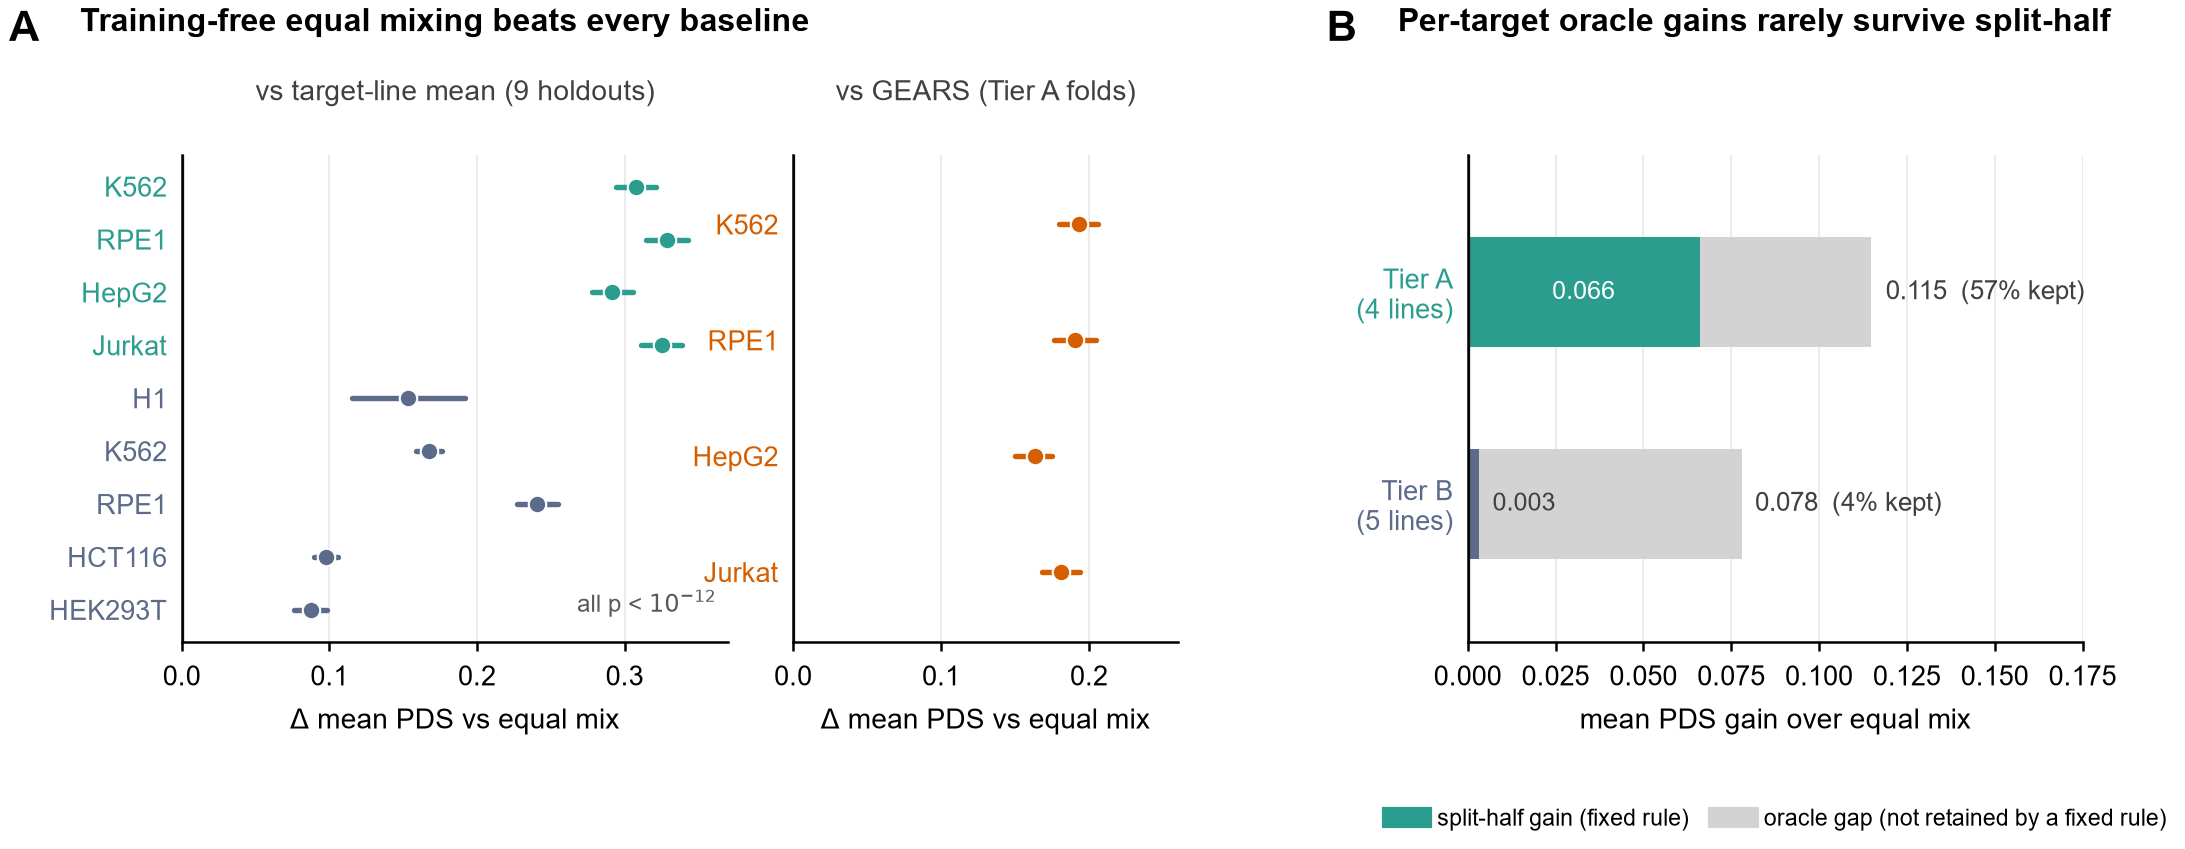
\includegraphics[width=\textwidth]{graphical_abstract.png}
\end{center}

\doublespacing

\section{Introduction}

Perturbation screens have grown in scope. Libraries cover thousands of perturbations, and several cell lines are in common use [1–6]. K562 and RPE1 have genome-wide screens [1]. HCT116 and HEK293T entered through X-Atlas/Orion [7], and the 2025 Virtual Cell Challenge added H1 [8]. Nadig et al. put K562, RPE1, Jurkat, and HepG2 on one atlas [9]. If a perturbation has been measured somewhere, how much of that response survives a move to another line?

Benchmarks usually predict perturbations that were never measured, often across several contexts [10–14]. They do not have to strip every perturbed-cell label from the target line. The 2025 challenge kept 150 training, 50 validation, and 100 test perturbations and allowed expression atlases from other contexts [8]. Holding out an entire line is a different question [15]. That is the protocol here.

The first baseline uses no model. For a target measured in several source lines, unit-normalize each response and average them. That average predicts the held-out line. Nothing is fitted. The H1 cache is the exception: it comes from a fitted decoder, so not every upstream representation is training-free. Learned predictors should be compared on the same targets, with information access stated separately.

Scoring leaves room for shortcuts. A retrieval score ranks a prediction against a reference pool, and the target gene is usually knocked down in its own perturbation. Keeping that coordinate lets a prediction win by reproducing the knockdown. Absolute scores also move with pool size, target composition, and preprocessing; reporting choices can move them too. Keeping each target's best rule raises the mean, and so does scoring only the targets a method handles. Neither yields a deployable rule.

Two panels make this concrete. Tier A uses the four harmonized Nadig lines [9] on a shared 6,118-gene axis. Tier B brings H1, K562, RPE1, HCT116, and HEK293T from separate studies onto an 18,080-gene axis [1, 7, 8, 16]. One line is held out at a time, and its stored responses form the pool. A query needs a response in that line and at least one source. The retained set contains 5,486 Tier A and 18,678 Tier B queries.

We are not proposing a new predictor. We offer an evaluation protocol in three parts: a leave-one-line-out benchmark with two tiers; a rule-selection audit that reports the per-target oracle, the best fixed rule, and a split-half estimate as separate numbers; and within-panel diagnostics that test source-response agreement against retrieval and resample 50 scores to estimate where a panel sits when its reference pool is already measured.

\section{Results}

\subsection{Holding out a whole cell line isolates cross-line transfer}

The panels differ in how much preprocessing they share (Fig. 1; Table 1). Tier A uses the harmonized Nadig atlas [9]: four lines on a 6,118-gene axis, 5,952 evaluation positions, and 1,278 to 1,466 queries per holdout against pools of 1,340 to 1,537 targets. Tier B is a patchwork. H1 rows are decoded responses from the 2025 challenge [8]; K562 and RPE1 were profiled genome-wide [1]; HCT116 and HEK293T come from X-Atlas/Orion [7]. The five lines share an 18,080-gene axis with 10,778 finite positions. Coverage is uneven: 285 cached targets in H1 and 9,866 in K562, with 274 to 6,671 queries. The tiers contain 5,486 and 18,678 retained queries.

Each prediction is a signed response vector. The reference pool holds every stored response from the held-out line, including the query's own row. The task is to find the matching perturbation among the candidates. PDS compares the prediction with every reference by cosine similarity, then converts the matching response's rank into a percentile (Methods). The target gene's coordinate is removed from both sides. The benchmark measures matched-target transfer; unseen perturbations and gene-level accuracy are out of scope. For H1, the scoring reference is decoded, not measured.

\subsection{Equal mixing sets a high floor}

The target-agnostic mean lands near chance: mean PDS 0.499 to 0.537 and median 0.500 to 0.557 across holdouts (Table 2, Table S1).

Averaging the source responses for the same target is different (Fig. 1E, Fig. 2, Fig. 3C). Each source vector is unit-normalized before averaging, which keeps one line from dominating by scale. Mean PDS reached 0.794 to 0.829 in Tier A (median 0.918 to 0.985) and 0.590 to 0.744 in Tier B (median 0.639 to 0.848). The paired gain over the mean response was +0.292 to +0.329 in Tier A and +0.087 to +0.241 in Tier B, all $p < 5 \times 10^{-13}$ (Table S1). The mix won on 93–97\% of Tier A targets and 61–79\% of Tier B targets.

A single source competed but never reliably. In Tier B, equal mixing beat the best single source in every holdout, by 0.009 to 0.113 mean PDS. In Tier A, the best source beat equal mixing by 0.022 to 0.031 in three of four holdouts; equal mixing won by 0.031 in RPE1. That comparison is an oracle. Medians sit above means and the lower tail is heavy, so we report both.

\subsection{Reweighting and gating do not help}

We tested adaptive source weighting: raw mixing, top-2 source selection weighted by self-knockdown, similarity weighting at five temperatures, and ten aggregation variants (Methods). None raised mean PDS by more than 0.008; the best was +0.0075 for top-2 self-weighting in Tier A HepG2. Raw mixing lost up to 0.019 in H1 (Fig. 3A,B; Tables S1, S3).

The gate kept sources whose target-gene log fold-change was at most $-$1. Gated and equal mixing differed by at most 0.014 mean PDS; in Tier B the effect was $-$0.003 to +0.0004 and significant nowhere ($p = 0.24$ to 0.80; Table S6). Two Tier A effects were nominal and tiny ($-$0.008 in RPE1, $-$0.004 in HepG2). The unpaired version carries a selection confound, audited next.

\subsection{Per-target oracle gains differ from global rule-selection optimism}

A per-target oracle takes the best observed score for each target across candidate rules. That upper bound is not what one fixed rule delivers. We compared it with the best fixed rule and a split-half estimate over 200 draws; the half-sample protocol chooses one global rule on half the targets and scores it on the other half (Methods). Oracle minus best fixed is the heterogeneity gap. Best fixed minus split-half is global rule-selection optimism. The audit covers all nine holdouts and, separately, source selection in Tier A (Table S11; Fig. 9A).

Tier A had four mixing candidates. Per-target best-of scored 0.926 to 0.937 against 0.794 to 0.829 for equal mixing, an oracle gain of 0.101 to 0.132. The split-half gain was 0.032 to 0.094, all from mean centering; optimism was at most 0.0006. Nine Tier B candidates gave an oracle gain of 0.063 to 0.112 and a split-half gain of $-$0.005 to +0.021, positive only in RPE1. In H1 the oracle gained 0.112 while the global rule lost 0.005.

Source selection repeats the pattern (Table S11). On the 638 targets where equal mixing and all three single-source predictions exist, the best source per target reached 0.892 to 0.925, an oracle gain of 0.070 to 0.116; cross-fitting left an oracle gap of 0.060 to 0.100. The post-hoc best source in Section 2.2 was chosen once per holdout, not per target.

Gating raises a composition issue. Its gain splits into a composition term, equal mixing on the gate subset minus equal mixing on all targets, and a within-subset term. In Tier B these were +0.017 to +0.082 and $-$0.003 to +0.0004 (Fig. 9D). A gate keeps targets that are strongly knocked down in at least one source, and equal mixing already retrieves those easily. An unpaired gate table therefore books a composition effect as a method gain.

The Tahoe-100M panel is saturated. The per-condition oracle over eight budget rules moved mean PDS by $-$0.0015, and the best fixed and split-half rules each moved it by $-$0.006. The oracle-to-fixed gap grew with the number of candidates, from 0.008 to 0.014 in Tier A and 0.005 to 0.010 in Tier B, while the split-half gain stayed near zero (Fig. 9B,C). Reports of a per-target oracle should state the candidate count and coverage, and keep heterogeneity apart from global rule-selection optimism.

\subsection{Centering depends on the dataset}

Mean centering subtracts each source's mean response over its stored rows, renormalizes, then mixes equally. A shared stress or culture signature is not target-specific, but it can dominate the mixture. Centering helped in the harmonized tier: +0.089 in K562, +0.094 in HepG2, and +0.049 in Jurkat, all significant; RPE1 was +0.033 ($p = 0.56$). Four of five Tier B holdouts moved the other way ($-$0.027 H1, $-$0.035 K562, $-$0.037 HCT116, $-$0.005 HEK293T); only RPE1 improved (+0.021).

Target composition does not explain it. Query-matched centering, recomputing each source mean over the evaluated targets, kept the signs (Fig. 4B,C; Table S3). The sign follows the dataset and line pair. Centering has to be checked on the target dataset; it is not a default cleanup step.

\subsection{Scoring policy changes absolute scores, and can flip secondary effects}

Perturb a gene and its own transcript usually falls. With the target coordinate in, a prediction that reproduces the knockdown finds the true response easily. Exclusion asks whether the rest of the response is predicted.

We measured the shift in three Tier B holdouts with 1,000 sampled queries each (Fig. 5A,B; Table S5). Without exclusion, equal mixing reached median PDS 0.974 in K562, 0.928 in RPE1, and 0.884 in HCT116. With exclusion the medians fell to 0.765, 0.846, and 0.697. Stronger knockdowns lost more; the Spearman correlation with target-gene log fold-change was $-$0.55, $-$0.46, and $-$0.33 ($n = 784$, 828, and 528; all $p < 10^{-14}$).

The main result survived, but secondary conclusions did not always. Equal mixing still beat the mean response. In HCT116, centering went from +0.006 without exclusion to $-$0.028 with it. The 2026 Virtual Cell Challenge preset strips every panel target gene and uses denominator $n-1$ (Table S7). K562 lost 8,042 of 10,778 positions and HCT116 4,315. Equal-mixing scores fell only where thousands of genes were gone: K562 went from a mean of 0.677 to 0.577 and HCT116 from 0.635 to 0.606. The ranking held. Equal mixing beat the mean in all nine holdouts, by 0.299 to 0.335 in Tier A and 0.087 to 0.245 in Tier B (all $p < 10^{-12}$). Policy moves absolute scores, not the method ranking.

\subsection{Controlled predictions and pool composition audit the score}

We fixed 300 real queries per holdout and scored synthetic predictions with canonical PDS. The true response scored 1.000 by construction; a response from another query scored 0.513 in Tier A and 0.505 in Tier B; the target-agnostic mean scored 0.501 and 0.504; sign-reversed truth landed at 0.001. Equal mixing scored 0.812 and 0.654, close to the benchmark means (Table S21). Two controls behaved less cleanly. Gene-shuffled truth scored 0.655 in both tiers, and truth plus independent noise scored 1.000 at every level. PDS separates a truth-like direction from unrelated rows, but it is coarse.

Pool composition moved absolute PDS further than any method. On the 638-query panel we resampled 50- and 100-row pools from seven compositions and scored the same four predictions (Table S22). At 50 rows, equal-mix PDS ran from 0.438 in hard pools to 0.996 in easy pools, against 0.811 on the full pool. Random pools matched the full-pool level. Coherent and strong pools lowered equal mixing to 0.689 and 0.680; incoherent and quiet pools raised it to 0.896 and 0.890. Centered mixing was steadier but fell below equal mixing in easy, incoherent, and quiet pools. Method ranks flipped. A PDS level is conditional on its pool.

\subsection{Simple source statistics do not predict transfer}

Which source–target pairs transfer well? Single-source predictions gave a first look (Fig. 5C,D; Table S2). Response magnitude correlated positively with PDS in all 12 Tier A pairs ($\rho = +0.064$ to +0.416, median +0.298) and in 18 of 20 Tier B pairs ($\rho = -0.202$ to +0.463, median +0.134). Both exceptions were RPE1-as-source pairs.

Knockdown strength was weaker and less consistent: positive in 2 of 12 Tier A pairs and 2 of 20 Tier B pairs, with median $\rho$ of $-$0.05 and $-$0.10. The decile curve was not monotonic. Source statistics alone do not explain transfer.

\subsection{An independent H1 truth table leaves the tier level intact}

Of the 285 cached H1 rows, 150 are official challenge training targets. They have a DESeq2 pseudobulk log fold-change table that the benchmark never used. We reran the same queries and pools against that second truth, so only the truth changed. Prediction methods were defined on 141 of the 150 targets. Equal mixing scored 0.6532 against the cache and 0.6465 against DESeq2 clipped at $\pm 10$. Raw truth gave 0.6548 and a $\pm 5$ clip 0.6364. The paired difference was $-$0.0068 (95\% CI $-$0.0742 to +0.0647; Wilcoxon $p = 0.945$), while the mean response sat at 0.5124. The equal-mix advantage held under both pipelines.

Target-level agreement was modest: per-target PDS correlated at Spearman +0.18 ($p = 0.031$). Replacing the 285 decoded H1 source rows with the 150 cache or DESeq2 rows changed the mix in the four holdouts where H1 is a source by at most 0.0009, and per-target Spearman stayed at 0.984 or above. A Hallmark analysis correlated the equal-mix profile with DESeq2 at +0.1266 over 141 targets, against +0.0469 for a derangement control (difference +0.0797; 95\% CI +0.0041 to +0.1566; $p = 0.046$). The check validates the tier-level result.

\subsection{The tested GEARS adaptation does not close the gap to equal mixing}

We ran a GEARS [12] adaptation on all four Tier A folds. Where a target was measured in several sources, one source row was held out for validation and kept out of the training mean; the rest were unit-normalized and averaged. Equal mixing used every source row; GEARS trained on the remaining rows. The cell-graph input was zero, which is an additive reparameterization under the tested loss (Methods). All 5,486 Tier A queries were scored against the same pool, exclusion, and denominator.

Equal mixing beat GEARS in every fold (Fig. 1F, Table S14). Mean PDS advantages ran from +0.163 in HepG2 to +0.193 in K562; median advantages were +0.108 to +0.142, and win rates 0.84 to 0.88. Every paired Wilcoxon test had $p < 10^{-135}$. Two extra seeds reproduced every fold, with within-fold seed SD at most 0.007 (Table S15). GEARS was not at chance. It beat the target-agnostic mean by +0.115 to +0.144, so the order was mean response $<$ GEARS $<$ equal mixing.

Rescoring with five pool-free metrics gave the same order (Table S16): cosine +0.063 to +0.110, Pearson +0.065 to +0.111, top-50 Jaccard +0.047 to +0.056, and relative MSE lower by 0.027 to 0.058. In RPE1 the mean response had the highest cosine and Pearson yet a PDS of 0.4995, because a constant prediction cannot tell candidates apart. PDS rewards discrimination against a pool, not alignment. This is a stress test, not a GEARS leaderboard entry. A stored scGPT comparison is in Supplementary Fig. S1 and Table S4.

\subsection{Supervision helps here and there, but not everywhere}

We asked whether labeled targets from the held-out line change the picture. The line's other stored rows are available for fitting, and five-fold cross-validation keeps each query's response out of training. We tested a linear map (PCA to 1,024 components, ridge without intercept), a $k$-nearest-neighbor residual map ($k = 25$), and a residual multilayer perceptron.

On Tier B, neither the linear nor the kNN map improved on equal mixing (Table S8). The linear map changed mean PDS by +0.005 in H1 (95\% CI $-$0.033 to +0.041; $p = 0.77$) and by $-$0.005 to $-$0.054 elsewhere; the kNN map improved nowhere. Tier A took to the linear map: +0.069 in K562, +0.086 in HepG2, and +0.065 in Jurkat, all 95\% CIs above zero; RPE1 was +0.007. The residual MLP rose in K562 in both tiers (+0.044 and +0.038), in HCT116 (+0.026), and in HepG2 (+0.012, seed-fragile); Jurkat was null. It lowered mean PDS in RPE1 ($-$0.084 and $-$0.100), H1 ($-$0.053), and HEK293T ($-$0.023). A second seed reproduced the K562 and HCT116 gains but not HepG2. Zeroing the target coordinate left the gains intact, and within-fold permutation removed them. Supervision is a separate regime, not a replacement for equal mixing.

\subsection{Representative calibration sets help in some PCA-ridge holdouts}

Another use of effort is to measure a few perturbations in the held-out line and fit a map from the source mixture. The budget is the number $k$ of target-line measurements. We used the PCA-ridge map and varied only the selection of calibration queries. Each holdout was split into calibration and evaluation sets three times, and selection contrasts use the corrected budget scorer.

At $k = 20$, taking the query nearest each $k$-means cluster center of the source mixtures beat random selection in all four Tier A lines: +0.031 in K562, +0.075 in RPE1, +0.053 in HepG2, and +0.056 in Jurkat ($p = 4.9 \times 10^{-27}$ to $1.8 \times 10^{-32}$; Fig. 6, Table 3). Four of five Tier B holdouts agreed, by +0.022 to +0.050; H1 was null (+0.0001; $p = 0.49$). Among the alternatives, disagreement and max-min diversity sat 0.18 to 0.43 below equal mixing, magnitude and shared-response heuristics trailed random, and D-optimal selection lost 0.302 against random in K562. Only $k$-means beat random consistently, and Tier B was tested at $k = 20$.

The advantage decayed as $k$ grew. In K562 the $k$-means gain fell from +0.031 at 20 to +0.014 at 50 and +0.004 at 100, turning negative at 200. RPE1 fell from +0.075 to $-$0.002 at 200. On the 638-query panel, $k$-means at 50 to 100 raised mean PDS in K562, HepG2, and Jurkat and lowered it in RPE1; at $k = 200$ random beat $k$-means in all four lines. Scoring policy decides whether this works. Under no-exclusion scoring the mean change was negative at every budget for both rules (Table S10), because the equal mix already carries the source knockdown.

\subsection{One source line and tens of calibration perturbations are partly exchangeable}

The second budget decision is whether to add a source line or more target-line perturbations. On the balanced 638-query panel, every non-empty subset of the other three lines formed an equal mix, and subsets with at least two sources were calibrated with $k$ target-line perturbations.

Adding source lines is a weak lever. Mean equal-mix PDS was 0.7898 with one source, 0.8054 with two, and 0.8127 with three, about +0.011 per line (Fig. 7A, Table 4). Which lines you add matters more. RPE1 improved from its best single source to the full mix (0.817 to 0.841); K562, HepG2, and Jurkat went the other way, and RPE1 added to a HepG2 mix lowered PDS by 0.036. Eight of twelve additions were positive. Two had a finite exchange rate: a gain of +0.0039 matched 49 random perturbations, and +0.0273 matched 87 $k$-means or 97 random. A new source line costs 1,340 to 1,537 perturbations, a 14- to 31-fold saving where both routes reached the same gain.

Choosing the line is harder. Treating each source as a pseudo-holdout ranked the actual gain at Spearman $\rho = +0.790$ ($p = 0.0022$) across 12 decisions, while overestimating its size (median +0.026 against +0.011). The ranking needs validation in new lines.

\subsection{A drug-response panel lies beyond the regime boundary}

The genetic analyses use target-coordinate exclusion and four harmonized lines. For a drug-panel test we chose seven cancer lines from Tahoe-100M [17], an atlas that extends earlier single-cell screens [18, 19] and the Connectivity Map [20, 21]. Intersecting 304 drugs at up to three doses left 648 conditions measured in all seven lines. Drug responses have no single target coordinate, so each line was scored by cosine PDS against the same 648 conditions, using the equal mix of the other six. The outputs were near the ceiling: mean PDS 0.970 to 0.994, median 0.998 to 1.000, and unique top matches covering 42\% to 61\% of conditions (Fig. 8A, Table 5).

A matched genetic comparison puts the gap on a scale. Without exclusion, the four Nadig lines reached 0.820 to 0.869; the drug panel's one-source mix already sits at 0.964. Adding sources did little, from 0.964 to 0.987, about +0.004 per line against +0.013 in the genetic panel (Fig. 8B).

Calibration did not rescue the panel. Holding out 162 conditions per line and fitting the same PCA-ridge map on $k$ of the other 486 lowered the mean at every budget: $-$0.033 at $k = 20$ with $k$-means and $-$0.006 to $-$0.013 at larger $k$; random selection was lower still. Six of seven lines lost PDS at every budget, and 47 of 48 intervals lay below zero. Source-side allocation lost its signal: across 420 decisions, pseudo-gain correlated with actual gain at $\rho = -0.031$, against +0.790 in the genetic panel.

Resampling 50 full-pool scores estimates the regime when the complete pool is measured. Of 50,000 drug-panel draws, 0.05\% fell below the post-hoc 0.92 threshold, against 0.17\% of Nadig draws above it (Fig. 8F). Expanding to twelve lines left the conclusion intact: mean PDS 0.964 to 0.997, calibration negative at every budget, and all eight original row-pooled intervals below zero (Tables S17, S18). These estimates describe the measured pools.

\subsection{Source-response coherence as a within-panel diagnostic}

For each query we summarized agreement among the unit-normalized source responses: mean pairwise cosine, minimum pairwise cosine, and the norm of the mean. Centered versions subtract each source's mean row first. These summaries use source rows only.

Coherence ordered targets by PDS within holdouts. Mean pairwise coherence was 0.21 to 0.25 in Tier A and 0.04 to 0.11 in Tier B; its per-target Spearman with equal-mix PDS was +0.40 to +0.50 in Tier A and +0.09 to +0.29 in Tier B, pooled +0.34 (Fig. 10A, Table S12). It is not a proxy for source count (+0.33 partial) or response strength (+0.25 controlling log response norm). Across the nine genetic holdouts, mean coherence correlated with mean equal-mix PDS at +0.70 ($p = 0.036$; Fig. 10B), but most of that is a between-tier contrast; within-tier orderings were inconsistent. The mix-truth cosine tracked PDS at +0.70 within holdout, coherence at +0.64. The rank-residual estimator gave $-$0.17 for coherence controlling alignment and +0.66 for alignment controlling coherence. Alignment needs the held-out response; coherence does not.

The drug panel sits at the low-coherence end, 0.135 to 0.144 across seven lines, with near-perfect retrieval. Its competitor tail is thin: the held-out cosine lay above each line's 99th competitor percentile, and 0.6\% to 3.0\% of competitors ranked above the truth. Tier A had a similar mean margin and a heavier tail (13\% to 18\%). Equal-mix PDS is a margin rather than an alignment; levels are panel-specific, and so is the 0.92 threshold. Baseline similarity did not order Tier B holdouts ($\rho = +0.60$, $p = 0.28$, $n = 5$).

\section{Discussion}

This paper is an evaluation study. Method effects are kept apart from scoring policy, target composition, and data provenance. Equal mixing led in all nine holdouts, and reweighting and gating added little.

Tier B carries decoded H1 responses from several challenge splits. Swapping in a DESeq2 table for 150 H1 targets moved the pooled equal-mix level by 0.007 or less and retained a Hallmark signal; target-level agreement was weak ($+0.18$). The check validates the tier-level result. What transfers here is a matched-target response. Unseen perturbations, combinations, and model families lie outside this scope; Section 2.11 adds target-line labels and is a separate regime.

Why should averaging win? Unit normalization keeps a loud source from owning the mixture, and weakly correlated noise may cancel across sources. Shared target-specific responses would survive. The mechanism is a hypothesis, consistent with both noise cancellation and shared target responses.

The gate kept targets that equal mixing already retrieved easily, so most of its gain came from composition. Best-of reporting picks each target's rule using held-out outcomes and cannot be deployed. Evaluation leakage is a known problem [22, 23]. The oracle--fixed gap is not selection bias; it records how observed preferences differ across targets, and noise can enter that record. Split-half evaluation found little optimism in Tier A.

Centering lifted PDS in three of four harmonized holdouts and was neutral or harmful in four of five heterogeneous ones; query-matched centering rules out a simple composition story. The default should be to leave it off. Keeping the target coordinate in the score inflated median PDS by up to 0.21 and flipped centering's sign in one holdout. A panel-wide variant closer to challenge scoring moved absolute scores while the ranking stayed put. Cross-study comparisons and thresholds need a fixed exclusion policy and a sensitivity check.

GEARS used measured Tier A responses but reserved source rows for validation and replaced the ontology graph with a gene-set graph. Targets, pools, and scoring were matched; the methods differed in the information they could access. It beat the target-agnostic mean but not equal mixing. The scGPT comparison, fine-tuned on K562 only, is in Supplementary Fig. S1, Table S4, and Supplementary Note 1.

Target-line labels define a different regime. A linear map raised mean PDS in three of four Tier A holdouts and did nothing on Tier B; a residual MLP helped K562 and HCT116 but hurt RPE1, H1, and HEK293T by up to 0.100. Within-fold permutation removed the MLP gains. A method that needs target-line labels has not shown training-free transfer. Calibration gains depend on the map, scoring policy, and holdout, and beating random is only half the test: a calibrated prediction must also beat the uncalibrated mix. Two of eight positive source additions had a finite exchange rate, at 49 to 97 labels, which measures labels under a convention rather than total cost.

Drug-panel retrieval came close to the PDS ceiling in seven lines and stayed there at twelve. The tested calibration rules lowered the panel mean. That ceiling belongs to the measured pools, not to expression prediction. Resampling 50 scores separated the panels at a post-hoc 0.92; the cutoff describes the measured pools.

Coherence summaries point to within-panel associations: pooled rank correlations $+0.34$ for genetic responses and $+0.30$ for drugs, with alignment-controlled values $-$0.17 and $-$0.35. The negative partials keep coherence on the descriptive side.

The protocol also audits this study. The panel set follows data availability, and the 0.92 threshold is reported as post hoc. Applied to the gate, the same decomposition assigns most of its apparent gain to target selection (Sections 2.3 and 2.4).

\subsection*{What we would ask of cross-line benchmarks}

The rules below are the ones we would apply to a new panel.

\begin{enumerate}
\item Report the training-free equal-mix baseline on matched sources, plus the target-agnostic mean. A model that cannot beat the mix has shown no incremental value; it may still show transfer against the mean.
\item Separate composition from rule selection. Score gated and equal mixing on the same targets. With $K$ rules on $n$ targets, report the oracle, the best fixed rule, the split-half estimate, and the draw count. Heterogeneity is oracle minus best fixed; optimism is best fixed minus split-half. No learned per-target selector without out-of-sample evaluation.
\item Validate centering per dataset and line pair; do not apply it by default. Query-matched centering diagnoses target-composition effects.
\item State the scoring policy, including target-coordinate exclusion, and report a second policy where possible. Do not compare absolute PDS across policies. Give coverage, pool size, and paired intervals.
\item Give every learned model the same targets, pool, and scoring policy. Start calibration with a small representative set and compare against both random and the uncalibrated mix. Report both routes of an exchange rate.
\item Measure the baseline in its actual pool. Resampling 50 existing scores estimates the level for that pool; any cutoff is post hoc. A prospective stopping rule would add 50 new measurements.
\item Keep coherence descriptive and within-panel. Pooled rank associations are $+0.34$ for genetic responses and $+0.30$ for drugs; the partial values use a standard rank-residual estimator.
\end{enumerate}

\subsection*{Scope and applicability}

The genetic benchmark covers single loss-of-function perturbations, and the drug panel adds dose conditions. Most response matrices are pseudobulk log fold-changes or differential-expression estimates; H1 is the exception, with scVI-decoded responses from several challenge splits. None of the matrices retains cell-state heterogeneity. Modality, time point, preparation, and gene coverage differ across datasets. Harmonization narrows the differences in Tier A; Tier B keeps them. Absolute PDS values therefore say nothing across tiers or studies; inside a tier they move with pool size, target composition, and exclusion policy.

The pool keeps the query's own stored response, and predictions cover targets measured in at least one source. The benchmark scores matched-target transfer, and PDS measures discrimination among reference responses. The scGPT comparison covers 93 targets and one fine-tuning setup. GEARS uses one modified configuration, reproduced with two extra seeds. The selection audit covers four to nine candidate rules and one global rule; oracle gaps combine heterogeneity with response noise. Calibration uses one map class, and Tier B was tested at $k = 20$. The drug panel is one atlas of seven to twelve cancer lines with one pseudobulk profile per condition. The 0.92 threshold is evaluated after the gap was observed, and full-pool resampling treats every held-out response as available. Bootstrap intervals condition on existing fits. Exploratory p-values are nominal; twelve of thirteen primary selection contrasts survive Benjamini--Hochberg correction, and H1 is null.

\section{Methods}

\subsection*{Data}

\textbf{Tier A.} The four-line Nadig atlas [9], harmonized across K562, RPE1, HepG2, and Jurkat. A shared 6,118-gene axis leaves 5,952 evaluation positions; responses are log fold-changes against control; each line is held out in turn.

\textbf{Tier B.} H1 enters through a cache associated with the 2025 Virtual Cell Challenge [8]. The cache has 285 target rows covering all 150 training targets, 35 of 50 validation targets, and all 100 test targets. A separate DESeq2 pseudobulk log$_2$ fold-change table covers the same 150 training targets. K562 and RPE1 come from genome-wide Perturb-seq [1]; HCT116 and HEK293T from X-Atlas/Orion [7]. All five were mapped onto an 18,080-gene axis with 10,778 finite positions.

\textbf{Tahoe-100M.} Seven cancer lines (A549, A498, HS-578T, HEC-1-A, J82, MIA PaCa-2, SK-MEL-2) from Tahoe-100M [17]; 648 conditions (304 drugs at up to three doses) were measured in all seven. A robustness panel added five lines, leaving 646 shared conditions across twelve.

\textbf{Response representation.} The benchmark stores signed response vectors. Orion provided differential-expression values; K562 and RPE1 responses were computed from matched controls. H1 is decoded: perturbed cells are encoded with scVI, a mean latent displacement is added to control latents, and the shifted controls are decoded, with a log ratio against decoded controls. The reference pool for each held-out line contains all stored target rows. A query has a row in the held-out line and at least one source, and its own row stays in the pool. Pool sizes and query counts are in Table 1.

\subsection*{Perturbation discrimination score}

For a query target $t$, let $y$ be its stored response in the held-out line, $\hat{y}$ the prediction restricted to the evaluation positions, and $R = \{r_j\}$ the unit-normalized reference responses. Let $c$ be the target gene's coordinate. We set $\hat{y}_c = 0$ and unit-normalize $\hat{y}$. For each reference row $r_j$, the cosine similarity in the subspace with coordinate $c$ removed is
\[
s_j = \frac{r_j \cdot \hat{y}}{\sqrt{1 - r_{j,c}^{2}}\,\lVert \hat{y} \rVert},
\]
With exclusion off, we unit-normalize $\hat{y}$ without zeroing and use ordinary cosine.

Let $s_t$ be the similarity of the true response. The tie-midrank is
\[
\mathrm{rank}_0 = \#\{j : s_j > s_t\} + \tfrac{1}{2}\bigl(\#\{j : s_j = s_t\} - 1\bigr),
\]
and the score is
\[
\mathrm{PDS} = 1 - \mathrm{rank}_0 / n,
\]
where $n$ is the number of reference rows [24]. PDS reaches 1 when the true response is the unique top match. The drug panel has no target coordinate and uses ordinary cosine.

Our score is a target-coordinate exclusion variant of the perturbation discrimination score used in recent virtual-cell evaluations [8]. The cell-eval2 preset for the 2026 Virtual Cell Challenge (version 0.18.0, commit 0ce25cf) excludes target genes panel-wide and uses denominator $n-1$. We keep target-coordinate exclusion because our pools contain all stored response rows. The convention changes absolute scores (Table S7).

\subsection*{Checks with pool-free metrics}

We rescored the GEARS predictions under five pool-free metrics: cosine with the target coordinate zeroed in both vectors; Pearson correlation of mean-centered vectors; top-50 Jaccard overlap by absolute value; relative mean squared error $\lVert\hat{y}-y\rVert^{2}/\lVert y\rVert^{2}$; and its scalar-calibrated form with $\alpha=\hat{y}\cdot y/\lVert\hat{y}\rVert^{2}$, a shape diagnostic that uses each query's truth. Paired differences use 4,000 bootstrap resamples and two-sided Wilcoxon tests.

\subsection*{Metric controls}

We fixed 300 uniformly sampled real queries per holdout; every stored reference row stayed in the pool. Synthetic predictions---true response, equal mix, target-agnostic mean, a deranged query's response, gene-shuffled truth, negated truth, and truth plus Gaussian noise at 0.25--4 times its norm---were scored with canonical PDS and summarized by cosine to the truth.

\subsection*{Pool composition control}

The balanced 638-query Nadig panel stayed fixed, together with its predictions and truths; only the competitor pool changed. At $m = 50$ and 100 rows, each pool held the true response plus $m-1$ candidates from one composition: random, hard or easy (most or least similar to the prediction), coherent or incoherent (source agreement), or strong or quiet (source norm). Candidate selection used source responses only. Fixed compositions used one pool per query; random pools were repeated 200 times. Scoring kept target-coordinate exclusion and tie midranks.

\subsection*{Predictors}

Let $S_t$ be the source lines with a stored response for target $t$, and $r_s(t)$ its response vector there. Every predictor returns a vector on the evaluation axis.

\begin{itemize}
\item \textbf{Mean response:} one vector over all stored source responses, used for every query.
\item \textbf{Single source:} the response $r_s(t)$ from one source $s$.
\item \textbf{Equal mixing:} $(1/|S_t|)\sum_{s \in S_t} r_s(t) / \lVert r_s(t) \rVert$.
\item \textbf{Raw mixing:} $(1/|S_t|)\sum_{s \in S_t} r_s(t)$.
\item \textbf{Mean centering:} with $\mu_s$ the mean response of source $s$ over its stored target rows, the prediction is $(1/|S_t|)\sum_{s \in S_t}(r_s(t) - \mu_s)/\lVert r_s(t) - \mu_s \rVert$.
\item \textbf{Query-matched centering:} $\mu_s$ is taken over the evaluated query targets available in source $s$.
\item \textbf{Gated mixing:} retain sources with self-log-fold-change $\le -1$, unit-normalize and average.
\item \textbf{Self-weighting:} the same gate, weighted by $-$self-log-fold-change.
\item \textbf{Top-2 self-weighting:} the two strongest-knockdown sources, weighted; equal weights if none is negative.
\item \textbf{Similarity weighting:} weights $\exp(\cos(\pi_{\text{held-out}}, \pi_s)/T)$ from log1p control profiles on shared expressed genes, $T \in \{0.05, 0.1, 0.2, 0.5, 1.0\}$; Tier B only.
\end{itemize}

Fixed-sample scans of 1,000 queries per holdout added best-self, consensus/medoid, norm weighting, coordinate-wise median, trimmed mean, and concordance weighting (Table S3).

\subsection*{Statistics}

Comparisons pair targets where both predictors are defined. We report the mean difference, a 95\% interval from 4,000 paired query bootstrap resamples, a two-sided Wilcoxon signed-rank p-value [25], and the win fraction. Genetic calibration scores are averaged within split and then by query identity across splits; bootstrap and Wilcoxon use these unique-query values. Fits, splits, and reference pools stay fixed, so intervals do not cover new lines or retraining. Exploratory p-values are nominal; 12 of 13 primary selection contrasts survive Benjamini--Hochberg correction [26] ($q \le 0.030$), and H1 is null. Gating has two components: composition is equal mixing on the gate subset minus equal mixing on all targets; mixing is gated minus equal mixing on the same subset.

\subsection*{Selection audit}

The audit reused per-target PDS values; no predictor was refit. For each holdout and candidate pool we formed a target-by-candidate matrix on targets where every candidate was defined. Let $O = \frac{1}{n}\sum_i \max_j s_{ij}$ be the per-target oracle and $F = \max_j \frac{1}{n}\sum_i s_{ij}$ the best fixed rule. The split-half protocol draws a random half $A$, selects $\hat{j}(A) = \arg\max_j \frac{1}{|A|}\sum_{i \in A} s_{ij}$, and scores it on the complement over 200 draws, following model-selection evaluations [27, 28]; $H$ is the mean complement score. We report heterogeneity $O-F$, optimism $F-H$, and oracle gap $O-H$. The split-half gain subtracts the equal-mix mean on the same evaluation half. Bootstrap intervals for $O-F$ use 1,000 target resamples. Candidate pools were equal, raw, mean-centered, and top-2 self-weighted mixing in Tier A; those plus similarity weighting at five temperatures in Tier B; single sources in Tier A on the 638-target panel; and eight calibration-budget rules for the drug panel. All draws used seed 0.

\subsection*{Target-coordinate sensitivity}

Three Tier B holdouts (K562, RPE1, HCT116) and 1,000 uniformly sampled queries per holdout; scores with and without exclusion under otherwise identical settings. The per-query drop was correlated with target-gene log fold-change (Spearman), with 1,000 bootstrap resamples.

\subsection*{H1 truth-pipeline confirmation}

A DESeq2 pseudobulk log$_2$ fold-change table covered the 150 official H1 training targets; the decoded cache covers 285, including those 150. We aligned both to the shared queries and scored the same source mixes against each truth, with queries and pools identical. The primary analysis clipped at $\pm 10$; raw and $\pm 5$ clips were sensitivities. Paired tests used 4,000 bootstrap resamples and two-sided Wilcoxon on 141 targets. We also scored the DESeq2 truth as a prediction against the full 285-row cache pool. For the source-table sensitivity, the 285 decoded source rows were replaced by 150 cache and then 150 DESeq2 rows. The pathway check averaged responses over the 50 Hallmark gene sets, removing the target gene from any set containing it, with a deranged-target control.

\subsection*{GEARS baseline}

GEARS [12] was adapted to the matched-target protocol on the Tier A axis, keeping the released model code and substituting a lightweight data object. The same pool and 5,952 evaluation positions held. When a target was measured in several sources, one source row went to validation and was excluded from the training mean; the rest were unit-normalized and averaged, and single-source targets contributed that row. Training used 1,949 to 1,961 targets with 1,508 to 1,591 validation rows. The cell-graph input was an all-zero vector, and the original ontology graph [29] was replaced by a substitute gene-set graph. Training used mean squared error and Adam; a documented check shows the zero graph input is an additive reparameterization under this loss. Predictions were scored with the same pool, exclusion, and denominator as equal mixing. Two extra seeds used the same configuration (Table S15); full settings are in the released scripts.

\subsection*{Supervised calibration}

Input was the equal-mix vector; the target was the unit-normalized held-out response. Models were fitted on the line's other stored rows in five folds. Three mappings were tested: PCA [30] to 1,024 components followed by ridge regression [31] without intercept (RidgeCV over 13 alphas from $10^{-2}$ to $10^{4}$), with a 256-component intercept variant; a $k$-nearest-neighbor residual map with $k = 25$ and softmax weights at $T = 0.1$; and a residual MLP (1,024 PCA components, hidden 512 and 256, GELU, dropout 0.1, AdamW at $10^{-3}$, batch 256, up to 60 epochs with early stopping). Sensitivity runs zeroed each target's coordinate or permuted response rows within training folds after the split, so no query's response could enter training under another label.

\subsection*{Calibration budget}

The same PCA-ridge map was used, varying only the calibration set. Tier A used all queries covered by the other three lines; three random splits assigned 300 queries to evaluation and the rest to calibration. Tier B used 137 evaluation queries for H1 and 200 for the others. Selection rules used source responses only: random; $k$-means [32] with the query nearest each center; shared, magnitude, agreement, disagreement, max-min diversity, greedy regularized D-optimal selection, and a diversity--disagreement hybrid. The map used PCA to $\min(1{,}024, |C| - 1)$ dimensions, ridge, and RidgeCV over the same alphas. $k$ was 5 to 200 where tested; random selection was repeated five times per split; zero crossings were interpolated over $k$.

\subsection*{External drug panel}

Prediction was the equal mix of unit-normalized responses to the same condition in the other six lines, scored against the line's 648 measured responses with ordinary cosine (no target coordinate). The same-drug control removed every candidate from the same line with the same drug name. Calibration split each line three times into 162 evaluation and 486 calibration conditions, using PCA to $\min(512, |C| - 1)$ dimensions, $k$-means or random selection, $k = 20$ to 200, and five random repeats. Source contributions were measured by removing each source and averaging the PDS change. Allocation covered 420 decisions. The full-pool pilot drew 50,000 samples of 50 computed query PDS values with replacement, keeping the original complete pool; it measures sampling variability, not 50 new measurements. The twelve-line panel repeated every analysis with eleven sources and 646 conditions.

\subsection*{Drug calibration interval sensitivity}

The sensitivity reuses stored condition-by-split deltas. Duplicate scores within a split are averaged first, then across available splits. Unique condition IDs are bootstrapped with 10,000 draws at seed 0, with shared weights across lines where supports align. A split-wise envelope uses $\alpha = 0.05/3$ over the three existing splits. Neither resplits nor retrains.

\subsection*{Small reference pools}

From the 638-target Nadig panel, each draw took $m = 50$ or 100 distinct targets without replacement; those targets supplied both queries and the whole held-out pool. Predictions were fixed before sampling. Reference-by-query cosine matrices were subset on both axes and tie-midranks recomputed with denominator $m$. Each size had 5,000 draws at seed 0, identical across lines and policies. Target-coordinate exclusion was applied to prediction and candidates with separate renormalization.

\subsection*{Source-coherence diagnostic}

For query $t$, let $u_s = r_s(t)/\lVert r_s(t) \rVert$ on the full stored axis. Mean pairwise coherence averages $u_s \cdot u_{s'}$ over source pairs; the minimum and the resultant $\lVert (1/|S_t|)\sum_s u_s \rVert$ are also reported. Centered versions subtract $\mu_s$ first. At least two sources are required. Raw associations use Spearman; partial associations use a standard rank-residual estimator (average ranks, ordinary least squares residuals on the covariate, Pearson on the residuals). Alignment is the cosine between the equal mix and the held-out response. Drug-panel partials are Fisher averages of the seven per-line values.

\subsection*{Reproducibility}

Derived data, predictions, per-target PDS values, and figure and table source data are in \texttt{outputs/}; analysis scripts are in \texttt{scripts/}. Figures are generated by \texttt{make\_figures.py}, \texttt{phase1\_budget\_curve.py}, \texttt{phase2\_exchange\_summary.py}, \texttt{make\_figures\_regime.py}, \texttt{selection\_figure.py}, and \texttt{make\_figure\_coherence.py}. Tables use \texttt{make\_tables.py}, \texttt{make\_tables\_budget.py}, and \texttt{make\_table\_regime.py}; the audit uses \texttt{selection\_audit.py}. The GEARS, secondary-metric, Tahoe, small-pool, and sensitivity analyses have dedicated scripts and outputs listed in the repository. The panel-wide sensitivity follows cell-eval2 vcc2026 at commit 0ce25cf. Provenance notes are listed in Data and code availability.

\section*{Data and code availability}

Public datasets come from the original publications. Replogle et al. [1] for K562 and RPE1. Nadig et al. [9] for the harmonized four-line atlas. X-Atlas/Orion [7] for HCT116 and HEK293T. The Virtual Cell Challenge [8] for H1. Tahoe-100M [17] for the drug-response panel. The official Virtual Cell Atlas currently provides count matrices for the original H1 training, validation, and test panels. The local H1 cache contains decoded responses spanning all three panels, not training responses alone. Its production inputs, model, and complete logs are not part of the local snapshot. Derived benchmark files and analysis code are available at \url{https://github.com/zhuzhenghao-max/mixing-vs-selection} and archived at \url{https://doi.org/10.5281/zenodo.24223291}. The pretrained scGPT model is available from Cui et al. [10], and the GEARS code from Roohani et al. [12]. The fine-tuned scGPT checkpoints are not part of the local snapshot. Revised sensitivity files accompany the release.

\section*{Competing interests}

The authors declare no competing interests.

\section*{Funding}

This work was supported by the National Natural Science Foundation of China (Grant No. 12305381).

\section*{Acknowledgments}

The authors thank the organizers of the 2025 Virtual Cell Challenge for releasing H1 data.

\section*{Supplementary material}

Supplementary Figure S1, Tables S1--S22, and Supplementary Notes 1 and 2 are provided in a separate file.

\section*{Author contributions}

Zhenghao Zhu designed the study, performed all analyses, and wrote the manuscript. Di Cui supervised the study and revised the manuscript.

\section*{Key Points}

\begin{itemize}
\item A leave-one-line-out benchmark holds out a whole cell line and scores every prediction against the same targets, reference pool, and rule: 5,486 queries over four harmonized lines and 18,678 over five heterogeneous lines.
\item A training-free equal mix of matched source responses beat the target-agnostic mean in all nine holdouts, by 0.087 to 0.329 PDS, and beat a GEARS adaptation by 0.16 to 0.19 PDS in every Tier A fold.
\item Per-target oracle gains overstate what one rule delivers. Split-half evaluation retained 57\% of the oracle gain in the harmonized tier and 4\% in the heterogeneous tier, so report oracle and out-of-sample estimates in separate columns.
\item Pool composition moved the equal-mix level from 0.438 to 0.996 PDS, and scoring policy could reverse secondary effects. Report target composition, pool size, and exclusion rules next to the score.
\item Source-response coherence correlated with retrieval within a panel (+0.34 for genetic responses, +0.30 for drugs) but is descriptive; it orders targets within a panel.
\end{itemize}

\begin{singlespace}
\begin{thebibliography}{99}

\bibitem{r1} Replogle JM, Saunders RA, Pogson AN, et al. Mapping information-rich genotype-phenotype landscapes with genome-scale Perturb-seq. \textit{Cell}. 2022;185(14):2559–2575.e28. doi:10.1016/j.cell.2022.05.013.

\bibitem{r2} Dixit A, Parnas O, Li B, et al. Perturb-seq: dissecting molecular circuits with scalable single-cell RNA profiling of pooled genetic screens. \textit{Cell}. 2016;167(7):1853–1866.e17. doi:10.1016/j.cell.2016.11.038.

\bibitem{r3} Adamson B, Norman TM, Jost M, et al. A multiplexed single-cell CRISPR screening platform enables systematic dissection of the unfolded protein response. \textit{Cell}. 2016;167(7):1867–1882.e21. doi:10.1016/j.cell.2016.11.048.

\bibitem{r8} Norman TM, Horlbeck MA, Replogle JM, et al. Exploring genetic interaction manifolds constructed from rich single-cell phenotypes. \textit{Science}. 2019;365(6455):786–793. doi:10.1126/science.aax4438.

\bibitem{r13} Replogle JM, Norman TM, Xu A, et al. Combinatorial single-cell CRISPR screens by direct guide RNA capture and targeted sequencing. \textit{Nature Biotechnology}. 2020;38(8):954–961. doi:10.1038/s41587-020-0470-y.

\bibitem{r14} Frangieh CJ, Melms JC, Thakore PI, et al. Multimodal pooled Perturb-CITE-seq screens in patient models define mechanisms of cancer immune evasion. \textit{Nature Genetics}. 2021;53(3):332–341. doi:10.1038/s41588-021-00779-1.

\bibitem{r6} Huang AC, Hsieh THS, Zhu J, et al. X-Atlas/Orion: genome-wide Perturb-seq datasets via a scalable fix-cryopreserve platform for training dose-dependent biological foundation models. \textit{bioRxiv}. 2025. doi:10.1101/2025.06.11.659105.

\bibitem{r10} Roohani YH, Hua TJ, Tung PY, et al. Virtual Cell Challenge: toward a Turing test for the virtual cell. \textit{Cell}. 2025;188(13):3370–3374. doi:10.1016/j.cell.2025.06.008.

\bibitem{r7} Nadig A, Replogle JM, Pogson AN, et al. Transcriptome-wide analysis of differential expression in perturbation atlases. \textit{Nature Genetics}. 2025;57(5):1228–1237. doi:10.1038/s41588-025-02169-3.

\bibitem{r4} Cui H, Wang C, Maan H, et al. scGPT: toward building a foundation model for single-cell multi-omics using generative AI. \textit{Nature Methods}. 2024;21(8):1470–1480. doi:10.1038/s41592-024-02201-0.

\bibitem{r9} Ahlmann-Eltze C, Huber W, Anders S. Deep-learning-based gene perturbation effect prediction does not yet outperform simple linear baselines. \textit{Nature Methods}. 2025;22(8):1657–1661. doi:10.1038/s41592-025-02772-6.

\bibitem{r11} Roohani Y, Huang K, Leskovec J. Predicting transcriptional outcomes of novel multigene perturbations with GEARS. \textit{Nature Biotechnology}. 2024;42(6):927–935. doi:10.1038/s41587-023-01905-6.

\bibitem{r15} Lotfollahi M, Wolf FA, Theis FJ. scGen predicts single-cell perturbation responses. \textit{Nature Methods}. 2019;16(8):715–721. doi:10.1038/s41592-019-0494-8.

\bibitem{r16} Lotfollahi M, Klimovskaia Susmelj A, De Donno C, et al. Predicting cellular responses to complex perturbations in high-throughput screens. \textit{Molecular Systems Biology}. 2023;19(6):e11517. doi:10.15252/msb.202211517.

\bibitem{r5} Bunne C, Roohani Y, Rosen Y, et al. How to build the virtual cell with artificial intelligence: priorities and opportunities. \textit{Cell}. 2024;187(25):7045–7063. doi:10.1016/j.cell.2024.11.015.

\bibitem{r19} Luecken MD, Büttner M, Chaichoompu K, et al. Benchmarking atlas-level data integration in single-cell genomics. \textit{Nature Methods}. 2022;19(1):41–50. doi:10.1038/s41592-021-01336-8.

\bibitem{r12} Zhang J, Ubas AA, de Borja R, et al. Tahoe-100M: a giga-scale single-cell perturbation atlas for context-dependent gene function and cellular modeling. \textit{bioRxiv}. 2025. doi:10.1101/2025.02.20.639398.

\bibitem{r17} Srivatsan SR, McFaline-Figueroa JL, Ramani V, et al. Massively multiplex chemical transcriptomics at single-cell resolution. \textit{Science}. 2020;367(6473):45–51. doi:10.1126/science.aax6234.

\bibitem{r18} McFarland JM, Paolella BR, Warren A, et al. Multiplexed single-cell transcriptional response profiling to define cancer vulnerabilities and therapeutic mechanism of action. \textit{Nature Communications}. 2020;11(1):4296. doi:10.1038/s41467-020-17440-w.

\bibitem{r20} Lamb J, Crawford ED, Peck D, et al. The Connectivity Map: using gene-expression signatures to connect small molecules, genes, and disease. \textit{Science}. 2006;313(5795):1929–1935. doi:10.1126/science.1132939.

\bibitem{r21} Subramanian A, Narayan R, Corsello SM, et al. A next generation Connectivity Map: L1000 platform and the first 1,000,000 profiles. \textit{Cell}. 2017;171(6):1437–1452.e17. doi:10.1016/j.cell.2017.10.049.

\bibitem{r29} Kaufman S, Rosset S, Perlich C, et al. Leakage in data mining: formulation, detection, and avoidance. \textit{ACM Transactions on Knowledge Discovery from Data}. 2012;6(4):1–21. doi:10.1145/2382577.2382579.

\bibitem{r30} Kapoor S, Narayanan A. Leakage and the reproducibility crisis in machine-learning-based science. \textit{Patterns}. 2023;4(9):100804. doi:10.1016/j.patter.2023.100804.

\bibitem{r23} Järvelin K, Kekäläinen J. Cumulated gain-based evaluation of IR techniques. \textit{ACM Transactions on Information Systems}. 2002;20(4):422–446. doi:10.1145/582415.582418.

\bibitem{r24} Wilcoxon F. Individual comparisons by ranking methods. \textit{Biometrics Bulletin}. 1945;1(6):80–83. doi:10.2307/3001968.

\bibitem{r25} Benjamini Y, Hochberg Y. Controlling the false discovery rate: a practical and powerful approach to multiple testing. \textit{Journal of the Royal Statistical Society: Series B (Methodological)}. 1995;57(1):289–300. doi:10.1111/j.2517-6161.1995.tb02031.x.

\bibitem{r31} Varma S, Simon R. Bias in error estimation when using cross-validation for model selection. \textit{BMC Bioinformatics}. 2006;7(1):91. doi:10.1186/1471-2105-7-91.

\bibitem{r32} Ambroise C, McLachlan GJ. Selection bias in gene extraction on the basis of microarray gene-expression data. \textit{Proceedings of the National Academy of Sciences}. 2002;99(10):6562–6566. doi:10.1073/pnas.102102699.

\bibitem{r22} Gene Ontology Consortium. The Gene Ontology resource: enriching a GOld mine. \textit{Nucleic Acids Research}. 2021;49(D1):D325–D334. doi:10.1093/nar/gkaa1113.

\bibitem{r28} Wold S, Esbensen K, Geladi P. Principal component analysis. \textit{Chemometrics and Intelligent Laboratory Systems}. 1987;2(1–3):37–52. doi:10.1016/0169-7439(87)80084-9.

\bibitem{r26} Hoerl AE, Kennard RW. Ridge regression: biased estimation for nonorthogonal problems. \textit{Technometrics}. 1970;12(1):55–67. doi:10.1080/00401706.1970.10488634.

\bibitem{r27} Lloyd S. Least squares quantization in PCM. \textit{IEEE Transactions on Information Theory}. 1982;28(2):129–137. doi:10.1109/TIT.1982.1056489.

\end{thebibliography}
\end{singlespace}

\clearpage
\begin{singlespace}
\section*{Figure legends}

\noindent\textbf{Figure 1. Design of the two-tier benchmark and the main results.} (A) How a query is formed. Stored response vectors for a target in the source lines are unit-normalized, averaged, and used as the prediction for the held-out line. H1 vectors are decoded estimates, not direct pseudobulk measurements. PDS scores the prediction against every stored response in the held-out line's reference pool, with the target gene's own coordinate removed. (B) Retrieval pool size (open circles) and number of evaluable queries (filled circles) for each line, on a log scale. Lines are grouped by tier, and the dashed line separates Tier A from Tier B. (C, D) Number of shared targets between each held-out line (rows) and source line (columns) in Tier A (C) and Tier B (D). Numbers in parentheses are pool sizes. The color scale is shared and logarithmic. (E) Equal mixing minus the target-agnostic mean response for each of the nine holdouts, paired on common targets; whiskers are 95\% bootstrap confidence intervals. Circles mark Tier A and squares Tier B. (F) Equal mixing minus GEARS in the four Tier A folds, paired on common targets; whiskers are 95\% bootstrap confidence intervals. Positive differences favor equal mixing.

\begin{center}
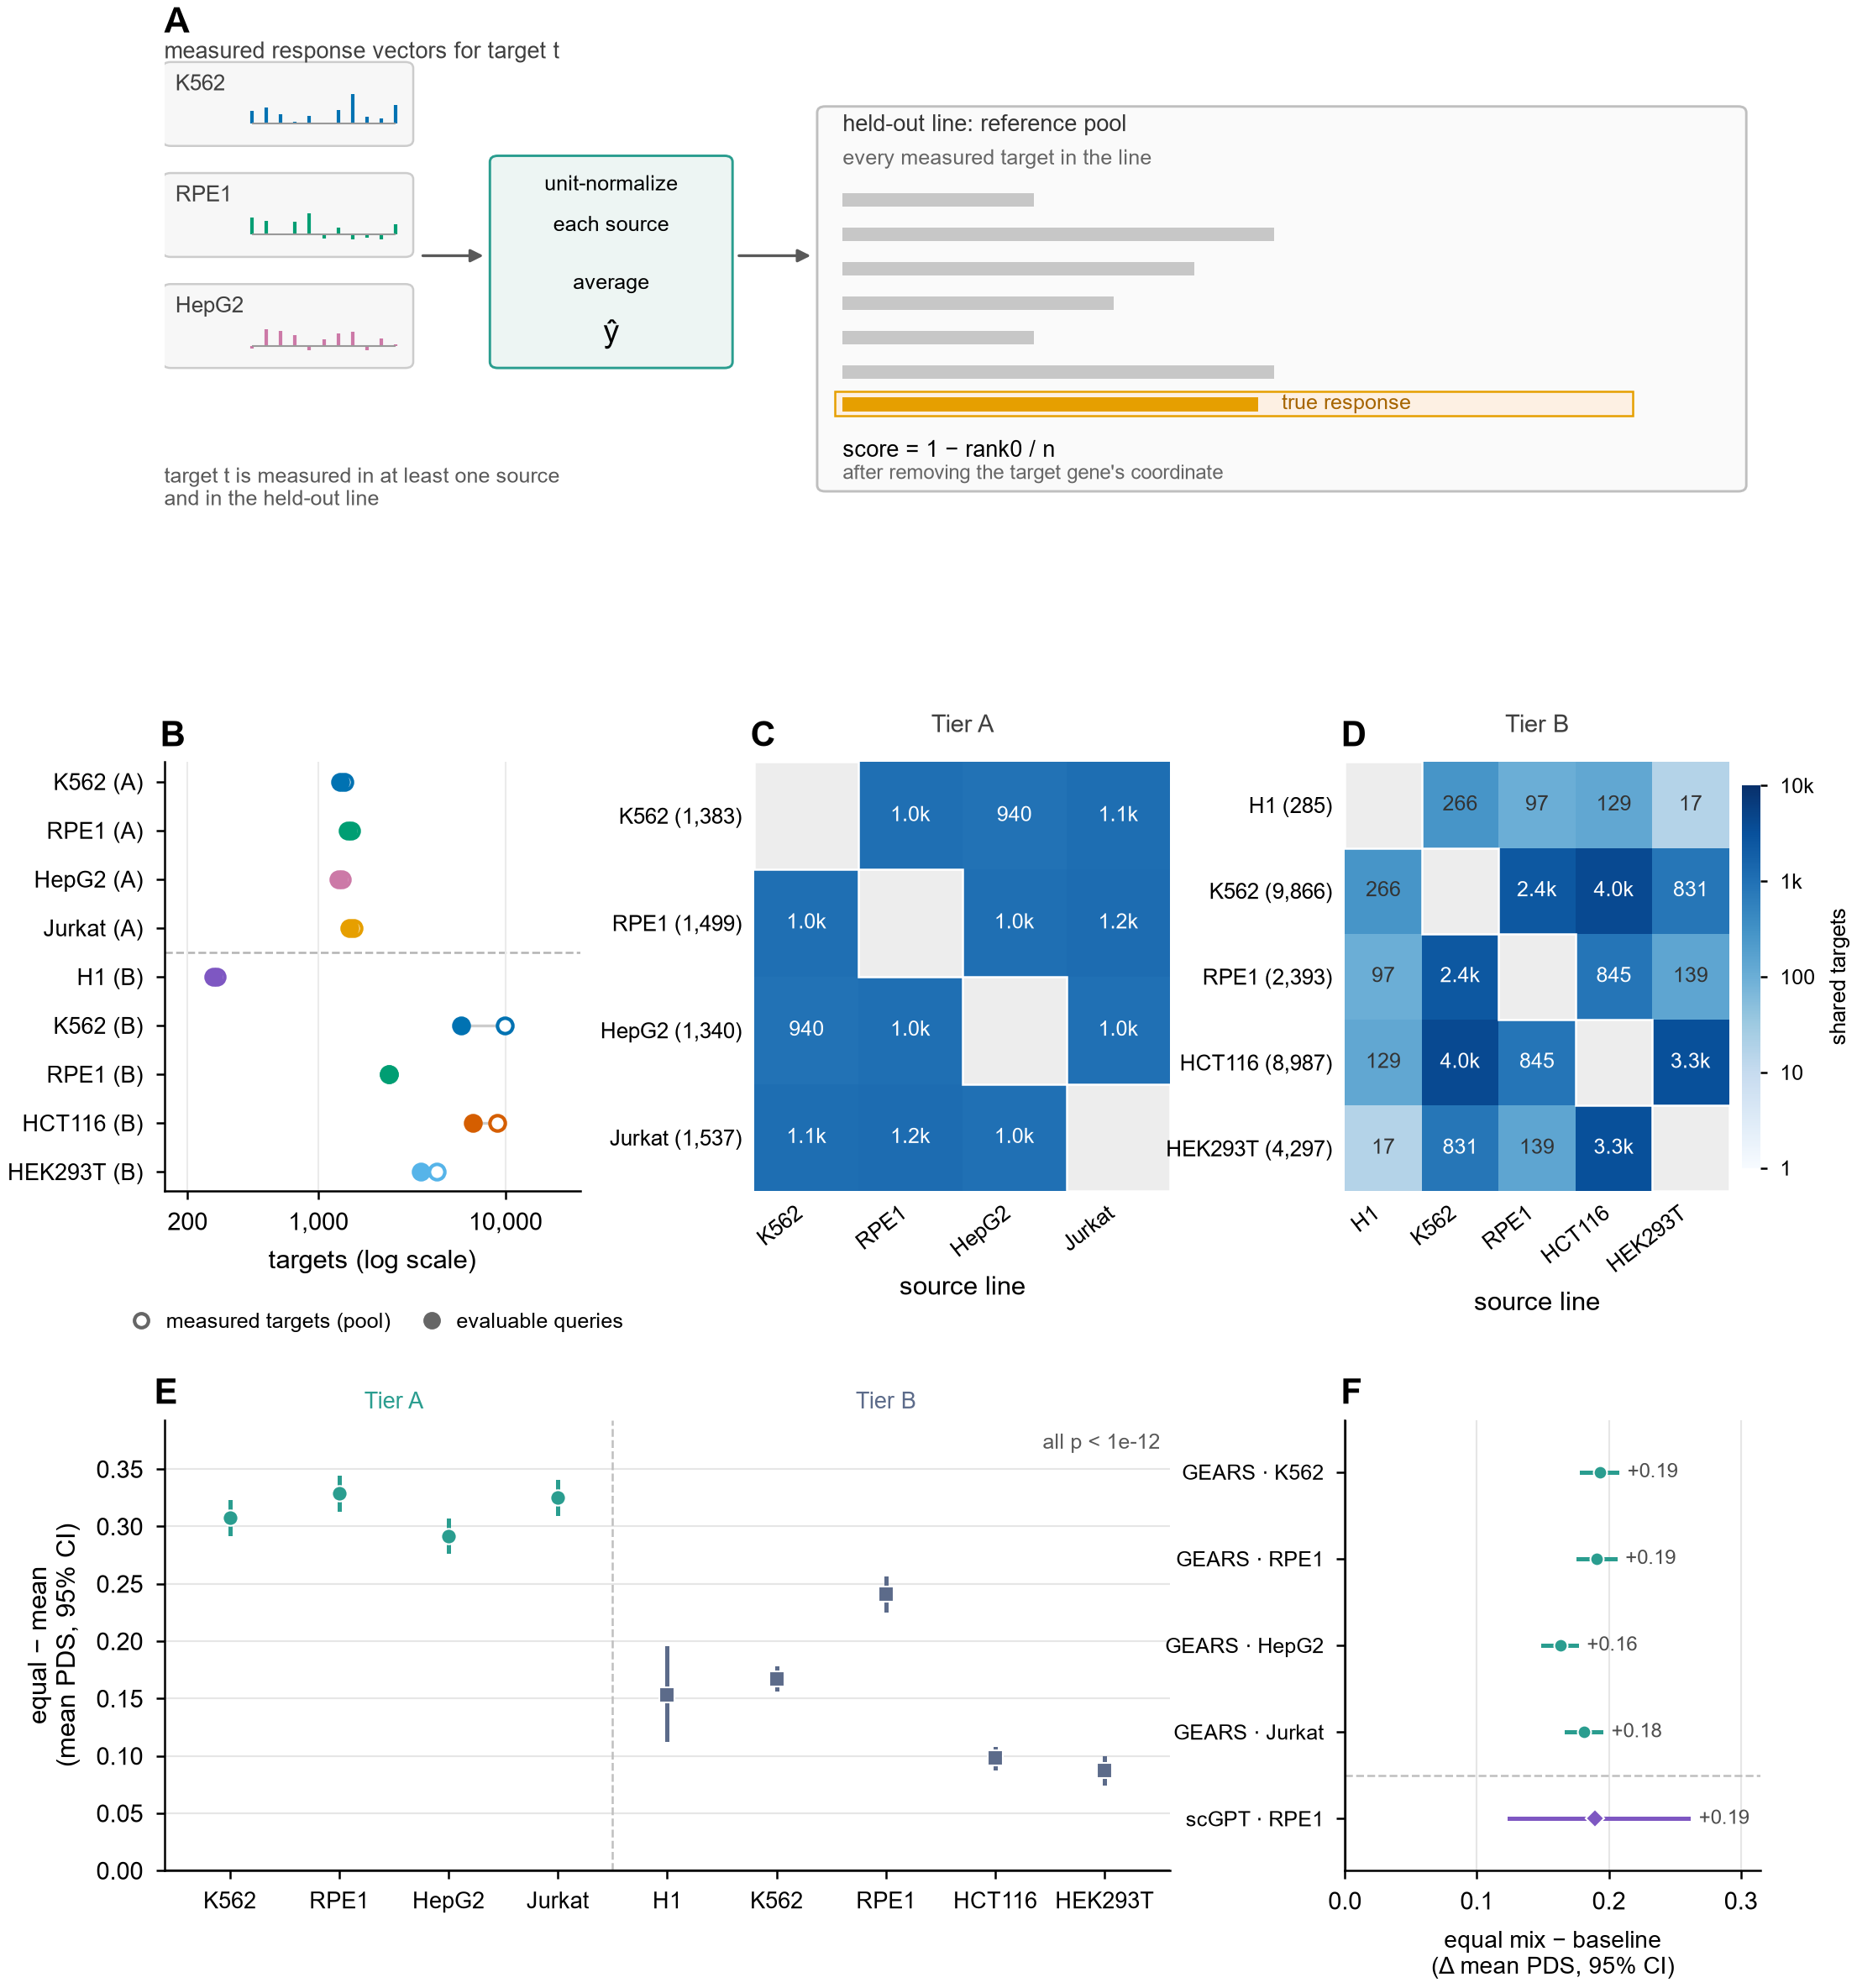
\includegraphics[width=\linewidth,height=0.68\textheight,keepaspectratio]{fig1_benchmark_overview.png}
\end{center}

\clearpage

\noindent\textbf{Figure 2. Mean and median PDS by method and held-out line.} (A) Mean PDS and (B) median PDS for each method (rows) and held-out line (columns). The vertical gap separates tiers. Best single source is chosen post hoc on held-out PDS and is an oracle reference. Cells show unpaired scores on each method's evaluable targets; paired comparisons on common targets are in Fig. 3 and Table 2. Absolute values depend on the exclusion policy (Fig. 5).

\begin{center}
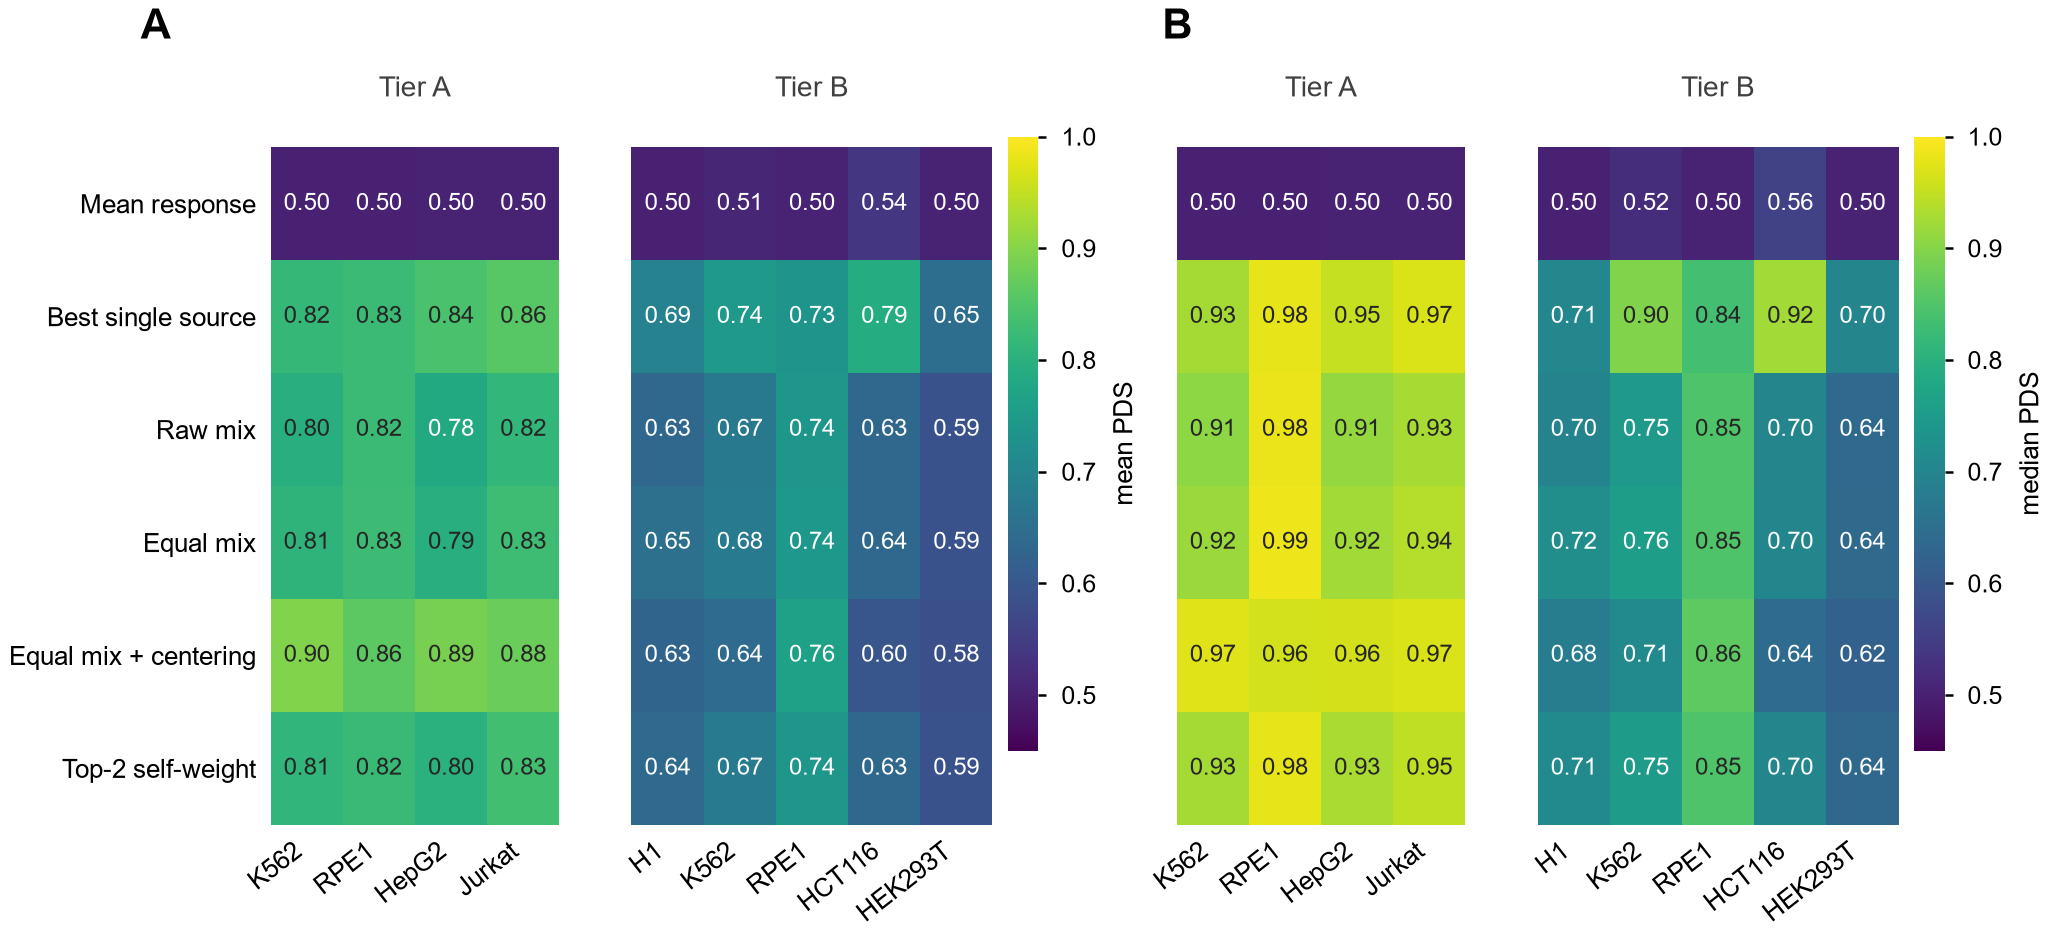
\includegraphics[width=\linewidth,height=0.68\textheight,keepaspectratio]{fig2_method_comparison.png}
\end{center}

\clearpage

\noindent\textbf{Figure 3. Paired comparisons against equal mixing.} (A) Tier A and (B) Tier B. Each dot is the mean paired PDS difference against equal mixing for one variant in one held-out line. Horizontal lines are 95\% paired-bootstrap confidence intervals. (C) Mean PDS gain of equal mixing over the target-agnostic mean response, all nine holdouts. Bars are 95\% paired-bootstrap confidence intervals. Every comparison has p < 10$^{-12}$ (two-sided Wilcoxon). In A and B, an interval that excludes zero generally means p < 0.05. Exact p-values are in Table S1.

\begin{center}
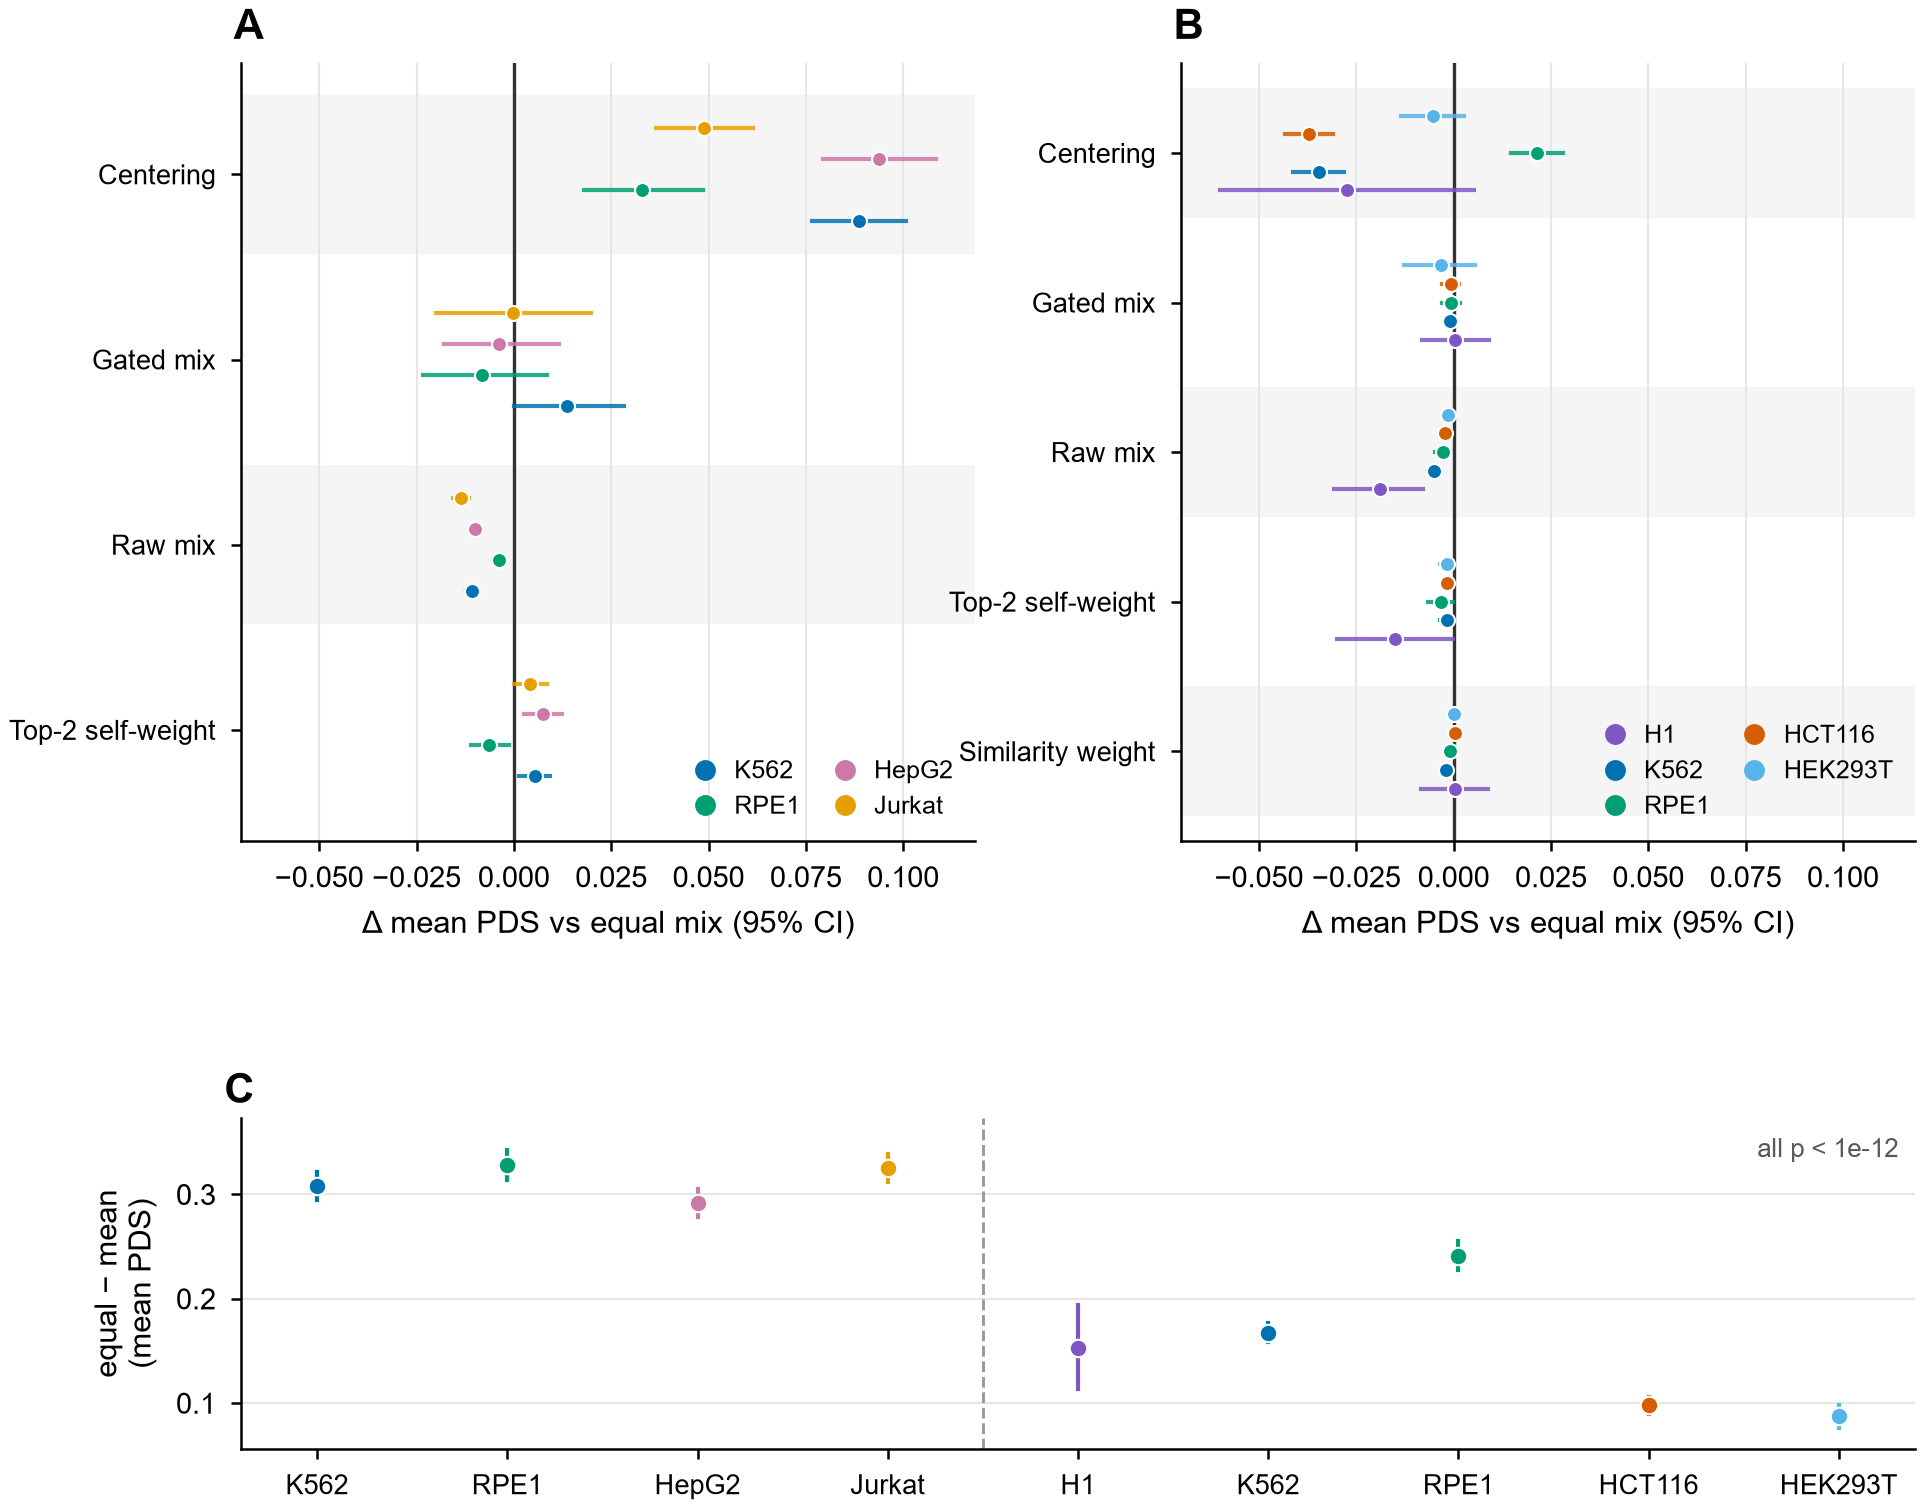
\includegraphics[width=\linewidth,height=0.68\textheight,keepaspectratio]{fig3_paired_deltas.png}
\end{center}

\clearpage

\noindent\textbf{Figure 4. Gating selects easier targets, and centering depends on the dataset.} (A) Decomposition of the gate effect. Blue bars give the selection effect, equal mixing on the gate-selected subset minus equal mixing on all targets. Orange bars give the gate effect, gated mixing minus equal mixing on the same gate-selected targets. Labels give the held-out line, tier, and gate/all target counts. (B) Mean paired difference in PDS between centering and equal mixing for each held-out line and tier; horizontal lines are 95\% paired-bootstrap confidence intervals. (C) Centering effect when the source mean is computed over the full source pool (open) or over the query targets only (filled), from the 1,000-query scan. Matching queries to targets does not remove the sign differences between lines.

\begin{center}
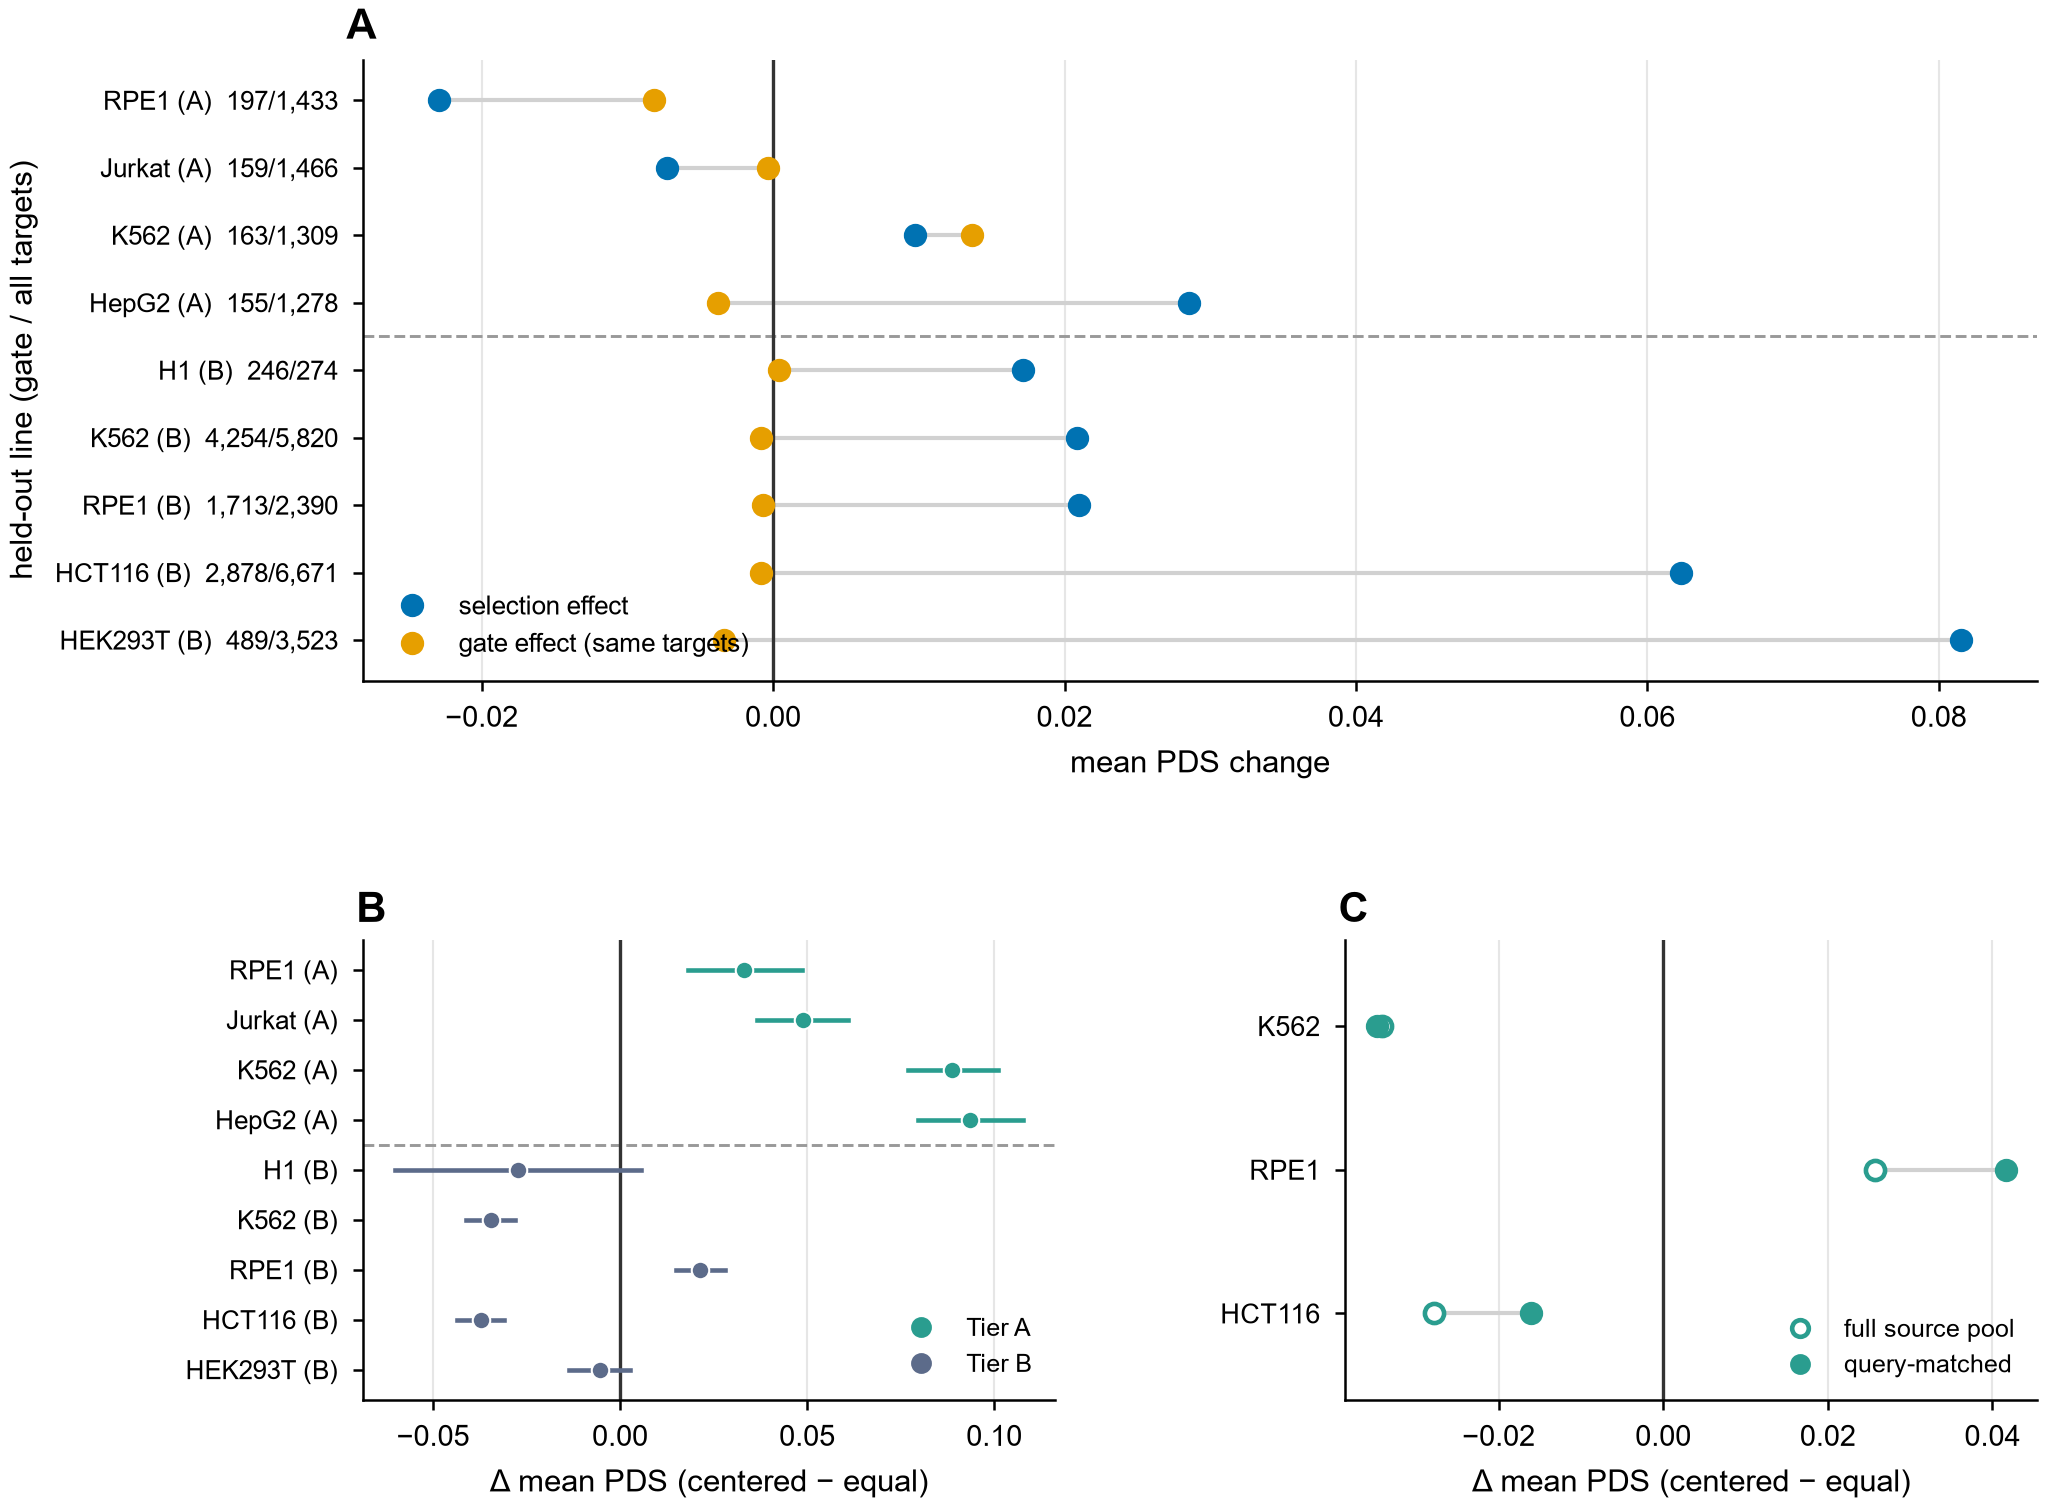
\includegraphics[width=\linewidth,height=0.68\textheight,keepaspectratio]{fig4_gate_and_centering.png}
\end{center}

\clearpage

\noindent\textbf{Figure 5. Metric sensitivity and what predicts transfer.} (A, B) Median (A) and mean (B) equal-mixing PDS in three Tier B holdouts, with target-coordinate exclusion (filled) and without it (open). Numbers mark the shift from no-exclusion to exclusion scoring. (C) Spearman correlation between single-source PDS and source response norm for every source–holdout pair, grouped by held-out line and tier. Pairs with fewer than 20 shared targets are omitted. That removes the two H1–HEK293T pairs (17 targets each) and leaves 16 of 18 positive Tier B pairs in the panel. The two negative pairs are H1←RPE1 and K562←RPE1. (D) Median PDS by self-log-fold-change decile within each source–holdout pair, averaged over pairs with at least 50 targets. Shading is $\pm 1$ SEM across pairs. Decile 0 has the strongest knockdown, decile 9 none.

\begin{center}
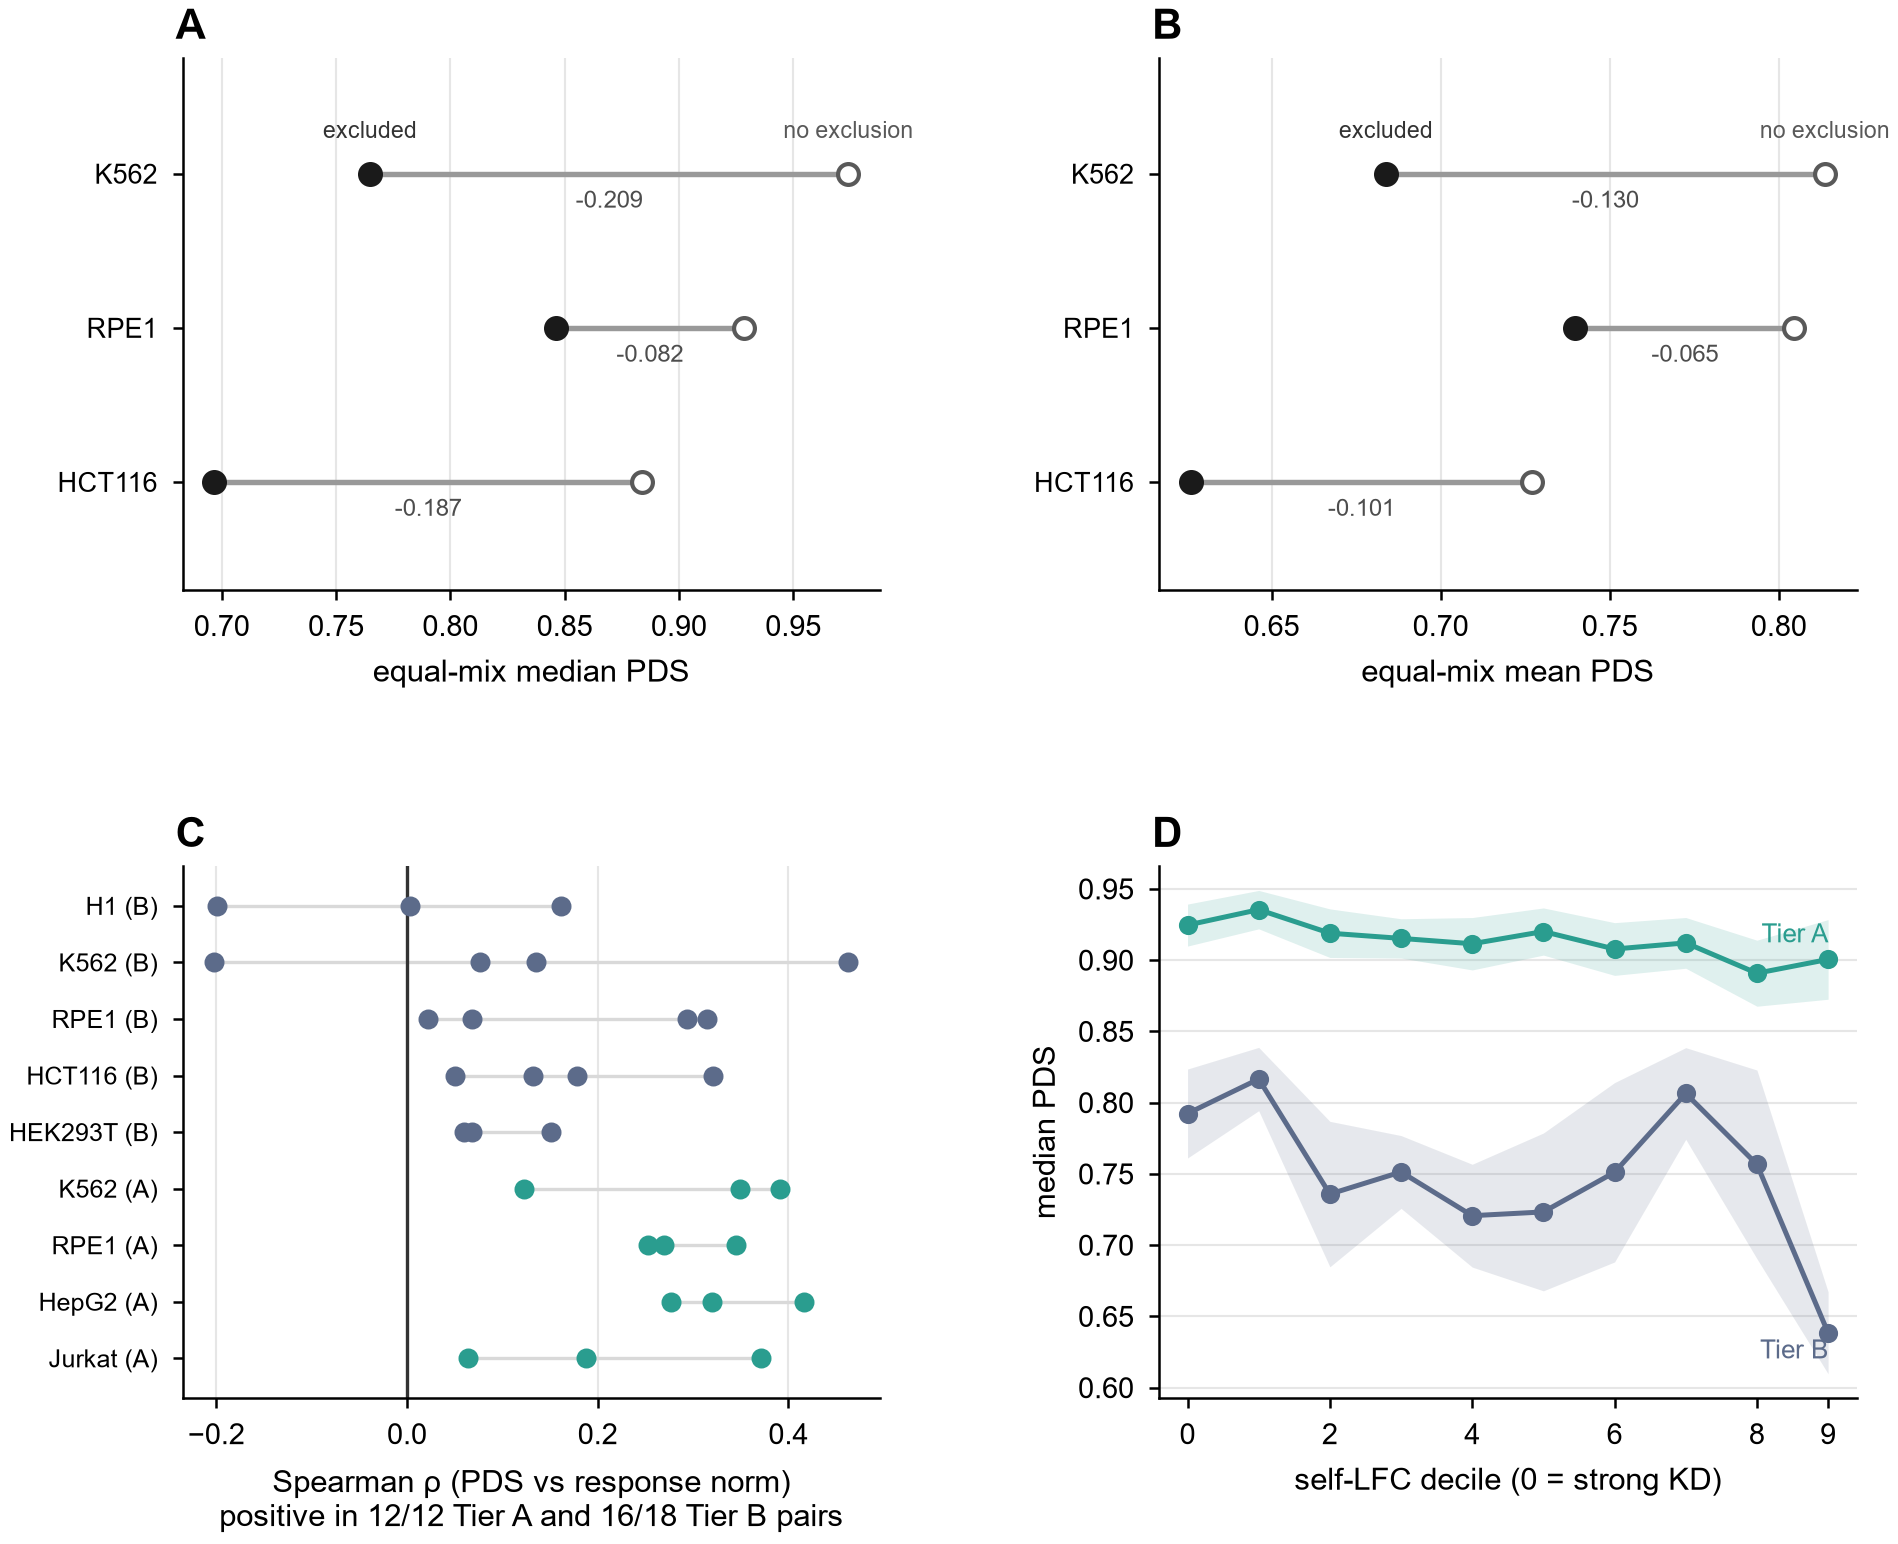
\includegraphics[width=\linewidth,height=0.68\textheight,keepaspectratio]{fig5_metric_determinants.png}
\end{center}

\clearpage

\noindent\textbf{Figure 6. Choosing calibration perturbations.} (A, B) Mean PDS change against equal mixing as calibration budget $k$ increases. K562 (A) and RPE1 (B), six selection rules. Negative values mean lower PDS than equal mixing. Points average three splits. Random selection is repeated five times per split. (C) The plotted point is the difference between $k$-means and random selection at each budget, with 95\% unique-query bootstrap intervals conditional on existing splits and fits. Repeated scores for each query are averaged before resampling, so the point and interval use the same paired query values. Re-splitting and retraining uncertainty are excluded. The $k$-means rule clusters source mixtures and takes the query nearest each center. Selection and fitting use source responses and the $k$ selected target-line labels. Evaluation also needs the full measured target-line reference pool.

\begin{center}
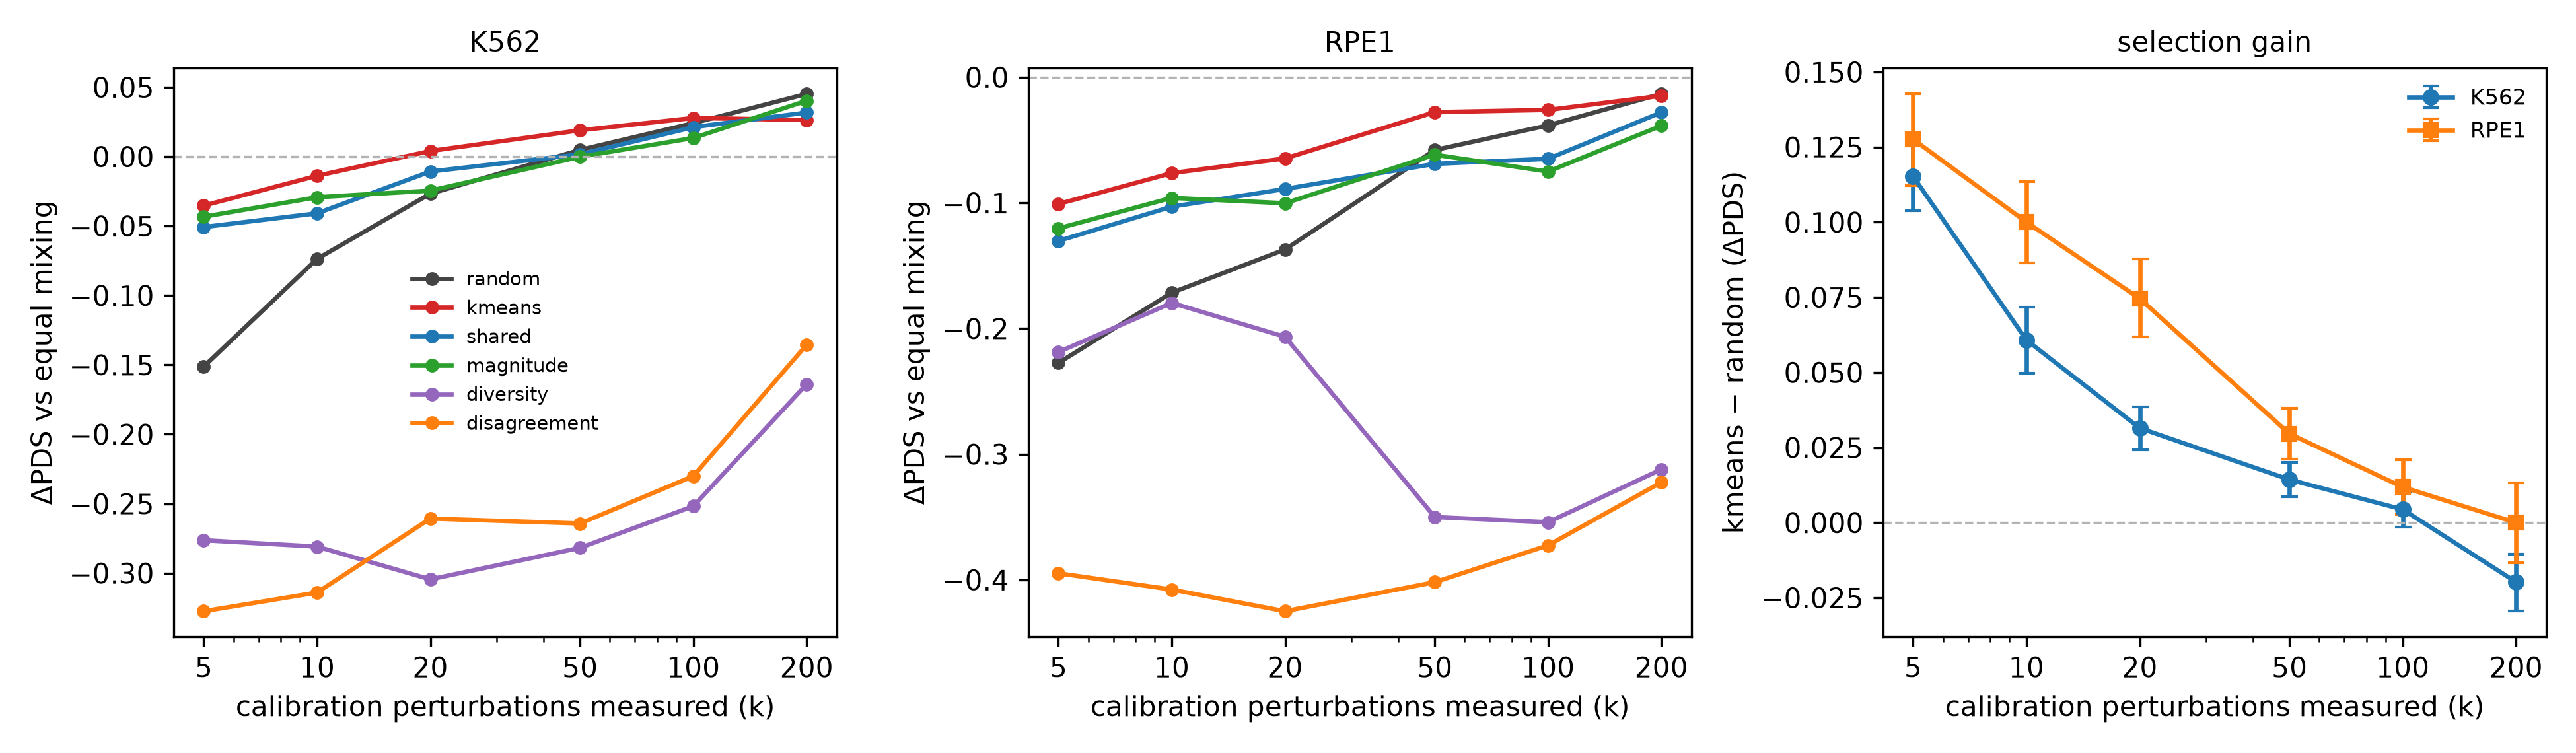
\includegraphics[width=\linewidth,height=0.68\textheight,keepaspectratio]{fig6_calibration_selection.png}
\end{center}

\clearpage

\noindent\textbf{Figure 7. Source lines against calibration perturbations.} (A) On the balanced panel of 638 queries, equal-mix PDS for each non-empty subset of the three source lines in every Tier A holdout. Subset labels index the source lines as listed for that holdout in Table 4A, and 0-1-2 is the full mix. (B) Calibration curves at the full mix for k-means (solid) and random (dashed) selection. (C) Exchange rate for source additions with a positive gain: the number of calibration perturbations needed to produce the same PDS gain as the added source line. Circles mark k-means, squares random, and triangles cases where the calibration curve did not reach the source gain within k = 200.

\begin{center}
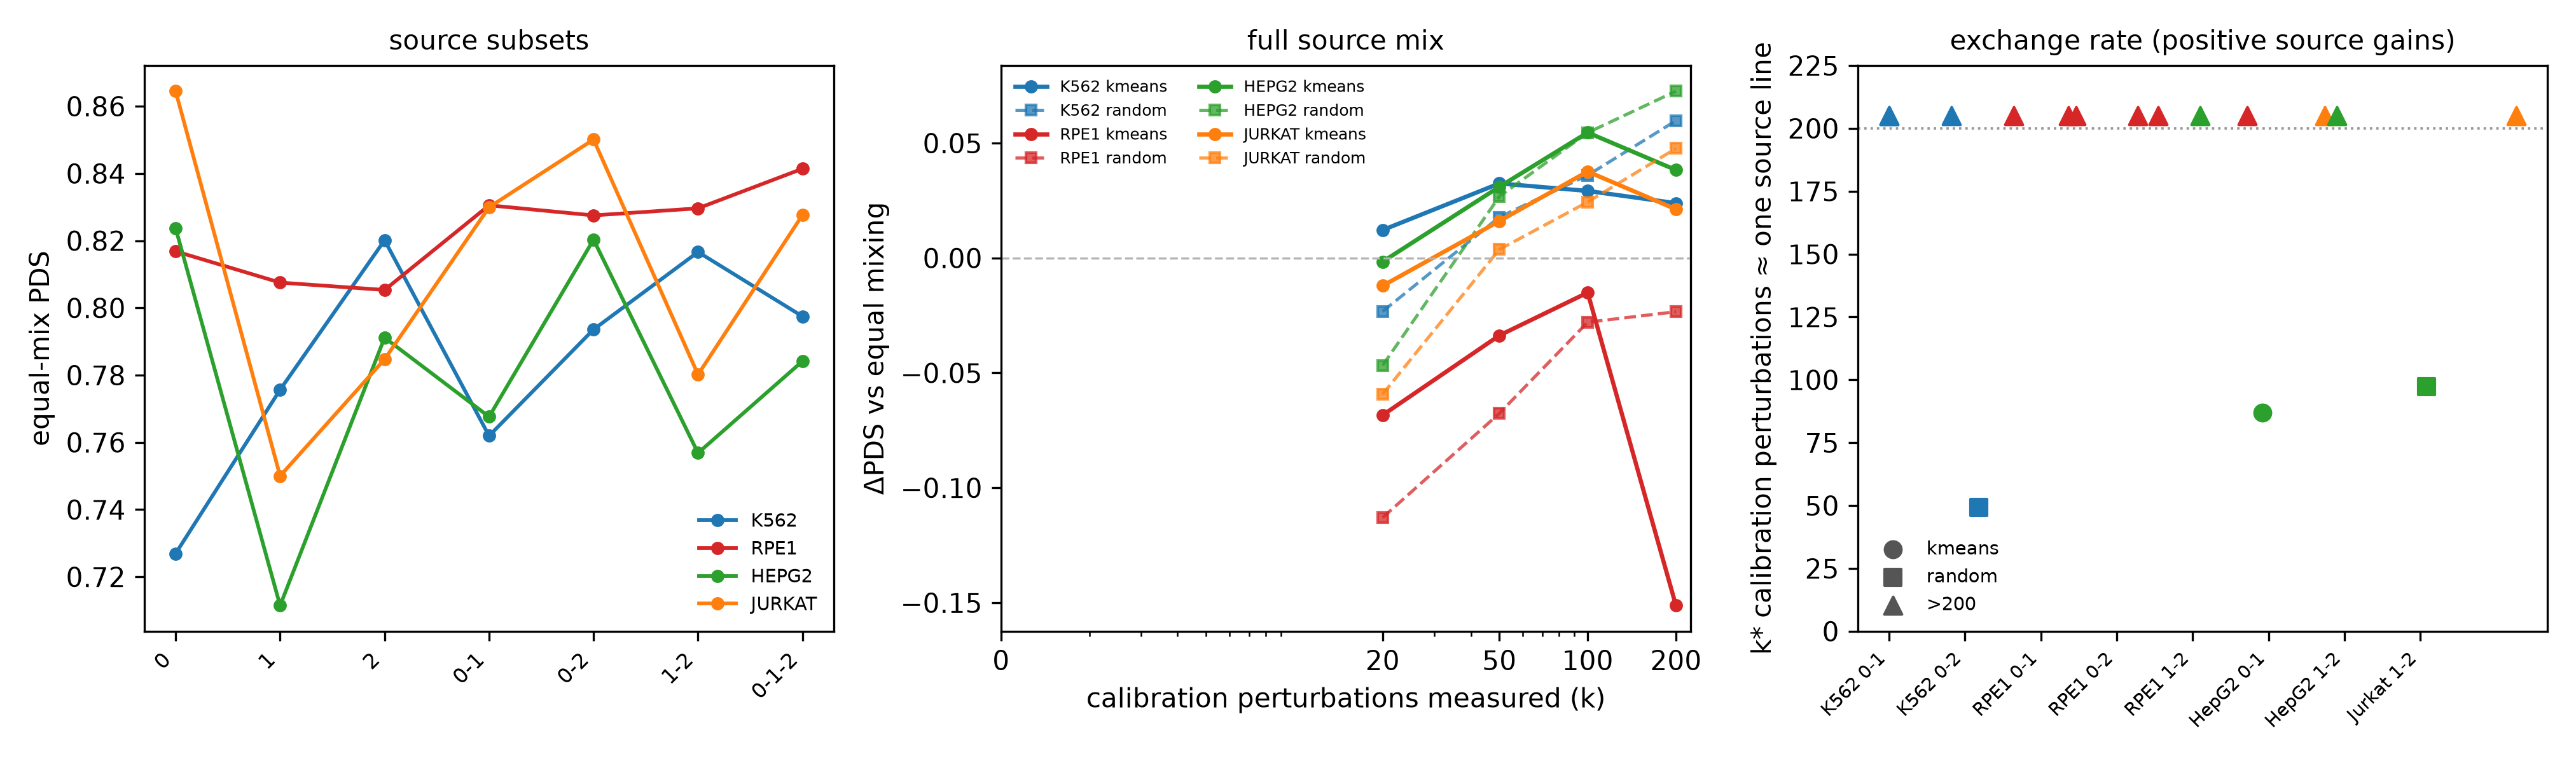
\includegraphics[width=\linewidth,height=0.68\textheight,keepaspectratio]{fig7_source_budget.png}
\end{center}

\clearpage

\noindent\textbf{Figure 8. A saturated drug-response regime.} Nadig calibration, allocation, and exclusion-scored pilot results use the corrected scorer. Tahoe scores come from the regenerated per-condition table; rebuilding the per-line response matrices requires the public Tahoe shards. (A) Cumulative distribution of per-query equal-mix PDS for the four Nadig lines under no-exclusion scoring (orange) and the seven Tahoe-100M lines (blue); thick lines pool the lines. (B) Mean PDS as a function of the number of source lines; Nadig uses no-exclusion scoring and Tahoe has no target coordinate. (C) Mean PDS change against equal mixing for k-means (solid) and random (dashed) calibration in each panel. Error bars are $\pm 1$ SD across lines; 95\% bootstrap confidence intervals for the panel means are reported in Section 2.14. Nadig uses target-coordinate exclusion on the balanced 638-query panel, while Tahoe has no target coordinate. (D, E) Pseudo holdout gain against actual source-add gain for Nadig (D) and Tahoe (E); the dashed line is equality. (F) Mean of 50 full-pool query scores sampled with replacement, from 50,000 draws per line; the dashed line marks the post-hoc 0.92 descriptive threshold. Each score uses the complete measured reference pool, not only the 50 sampled queries. Nadig uses target-coordinate exclusion, and Tahoe has no target coordinate. Panels A--F use the seven-line Tahoe panel; the twelve-line robustness panel is summarized in Tables S17 and S18.

\begin{center}
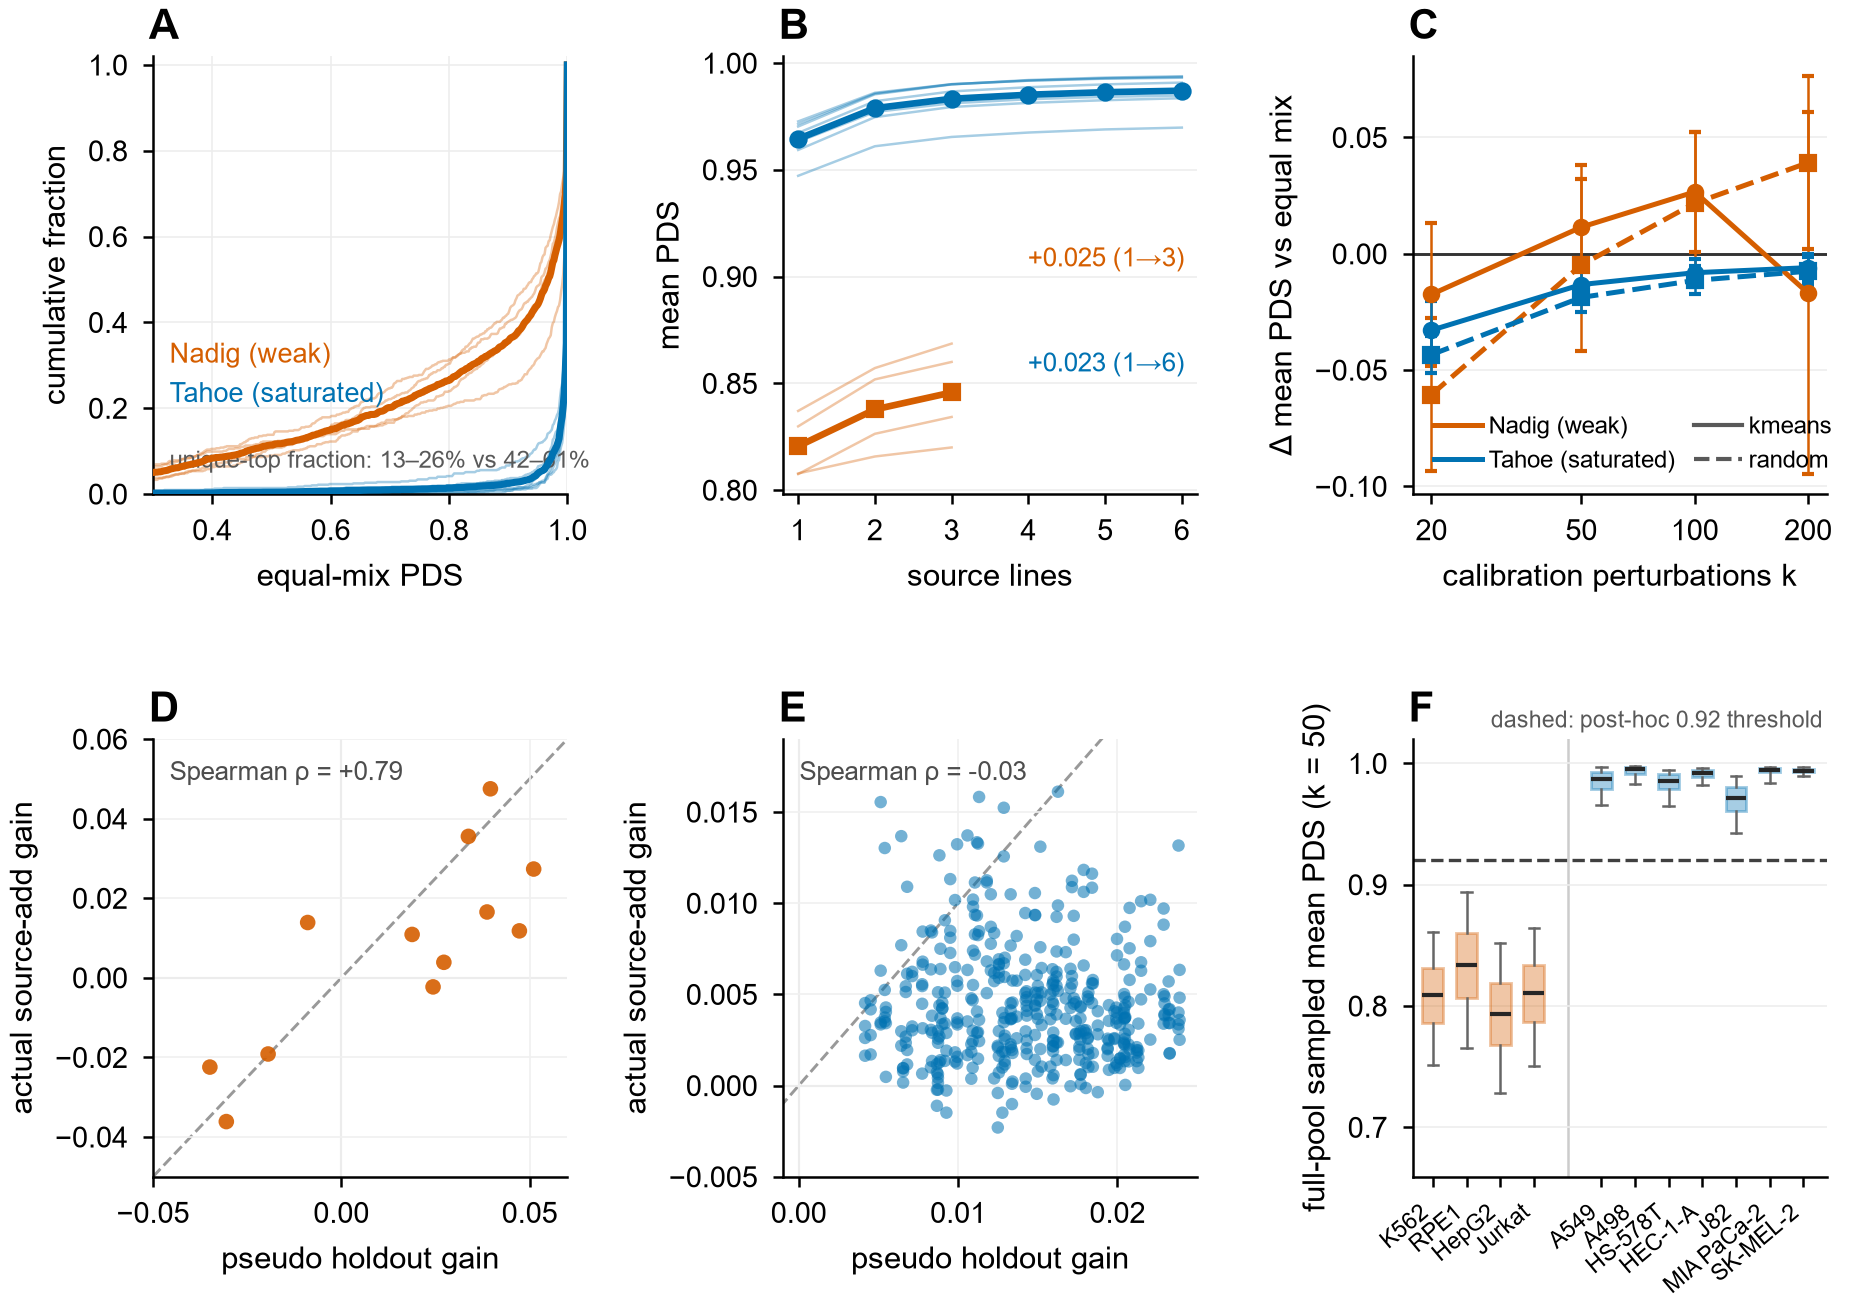
\includegraphics[width=\linewidth,height=0.68\textheight,keepaspectratio]{fig8_regime_boundary.png}
\end{center}

\clearpage

\noindent\textbf{Figure 9. Oracle gaps, global rule selection, and target composition.} (A) Bars show the per-target oracle minus the split-half estimate for one global rule in each holdout. This oracle gap does not estimate selection bias. Dots show the split-half gain over equal mixing. There are four rules in Tier A and nine in Tier B. Colors mark tiers. Bar plus dot equals the oracle gain over equal mixing. (B, C) Candidate-count curves for Tier A (B) and Tier B (C). Solid circles show oracle minus equal mixing. Dotted curves show best fixed rule minus equal mixing. Dashed squares show split-half gain. Oracle minus best fixed is the heterogeneity gap. Best fixed minus split-half is global rule-selection optimism. The Tier A pool excludes centering. No learned per-target selector is evaluated. (D) Gate decomposition. Composition is equal mixing on the gate subset minus equal mixing on all targets. Within subset is gated mixing minus equal mixing on the same targets. Their sum is the apparent gate gain.

\begin{center}
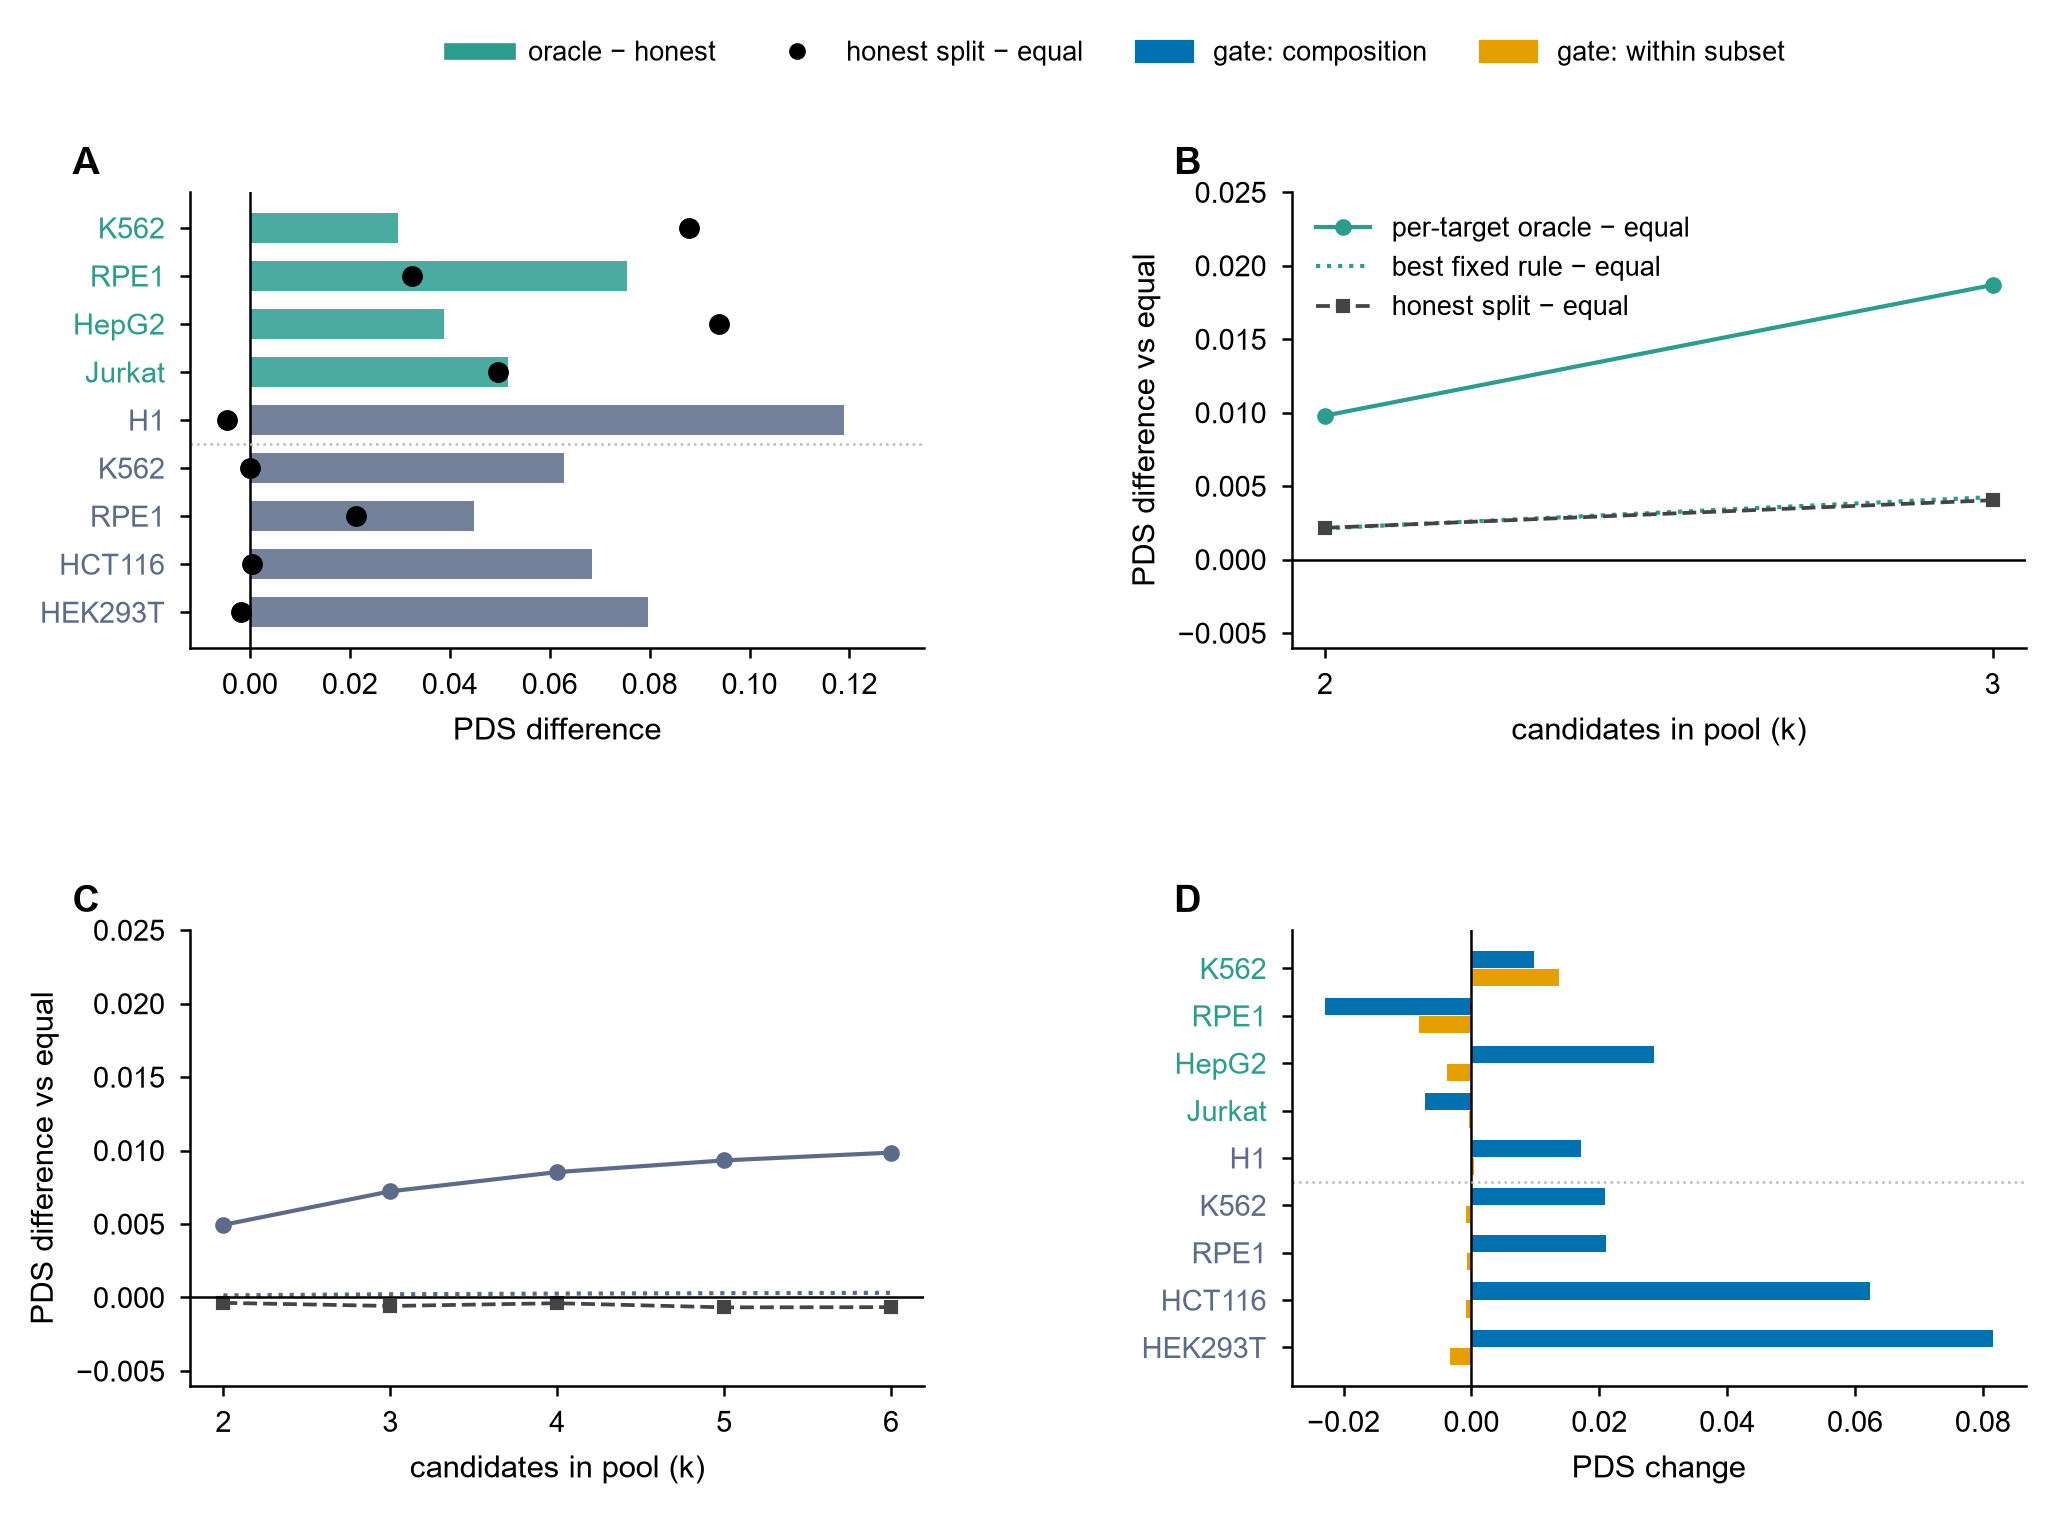
\includegraphics[width=\linewidth,height=0.68\textheight,keepaspectratio]{fig9_selection_audit.png}
\end{center}

\clearpage

\noindent\textbf{Figure 10. Source-response coherence analysis.} (A) Raw Spearman correlation between per-target source-response coherence and equal-mix PDS (filled), and the rank-residual partial statistic controlling log response norm (open), for each holdout. (B) Holdout-mean coherence against holdout-mean equal-mix PDS, for the nine genetic holdouts under target-coordinate exclusion (filled circles). The dashed line is a least-squares fit, and the annotation reports the Spearman correlation. Triangles mark the four Tier A holdouts scored without exclusion. Squares mark the seven drug-panel lines scored on the full pool, the policy appropriate when a panel has no target coordinate. The cross-panel ordering is descriptive. (C) Mean mix-truth cosine against source coherence, binned into within-tier quantile bins (eight per tier). Error bars are $\pm 1$ SEM of the bin mean, and the annotation is the mean within-holdout Spearman correlation. (D) Control-profile similarity between each Tier B holdout and its sources against equal-mix PDS. Coherence is the mean pairwise cosine of the unit-normalized source responses. Source-coherence summaries in A--C use source rows on queries covered by at least two sources. Held-out PDS, alignment cosines, and their associations use held-out responses. H1 rows are decoded estimates. These plots do not establish a mechanism.

\begin{center}
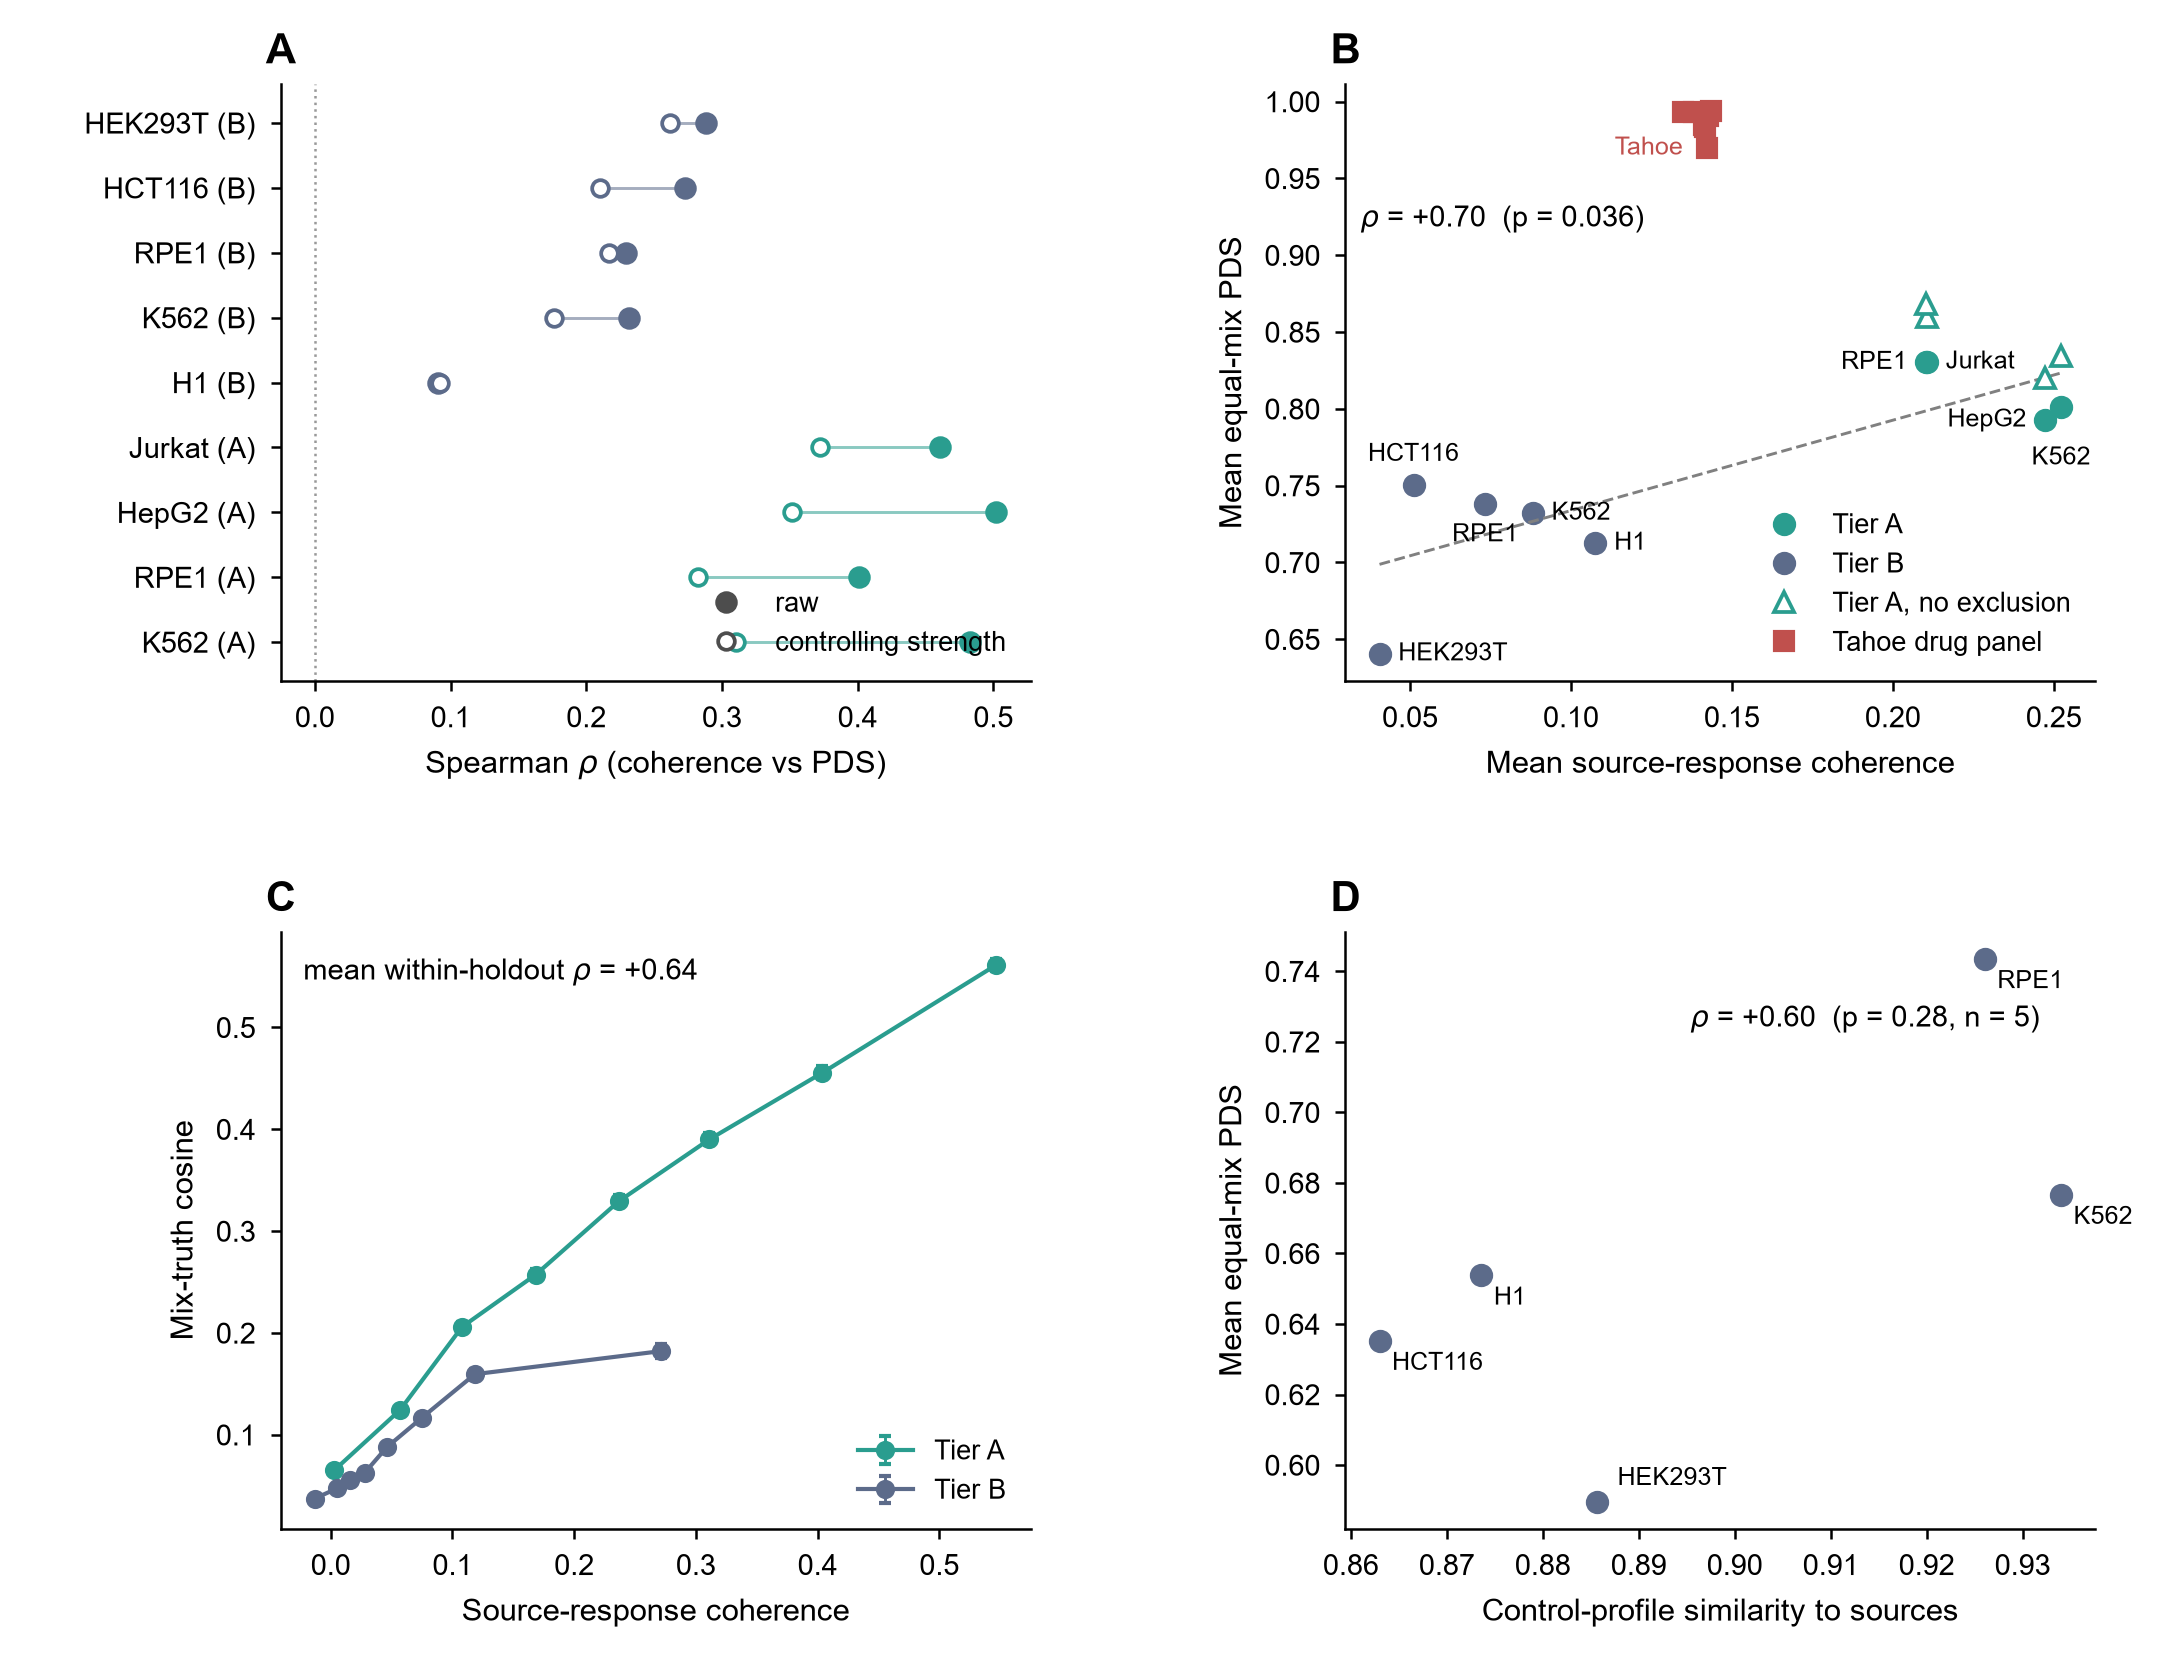
\includegraphics[width=\linewidth,height=0.68\textheight,keepaspectratio]{fig10_coherence_diagnostic.png}
\end{center}

\clearpage
\section*{Table legends}

\noindent\textbf{Table 1. Benchmark composition.} For each tier and held-out line the table gives retrieval pool size (stored target rows), number of evaluable queries, source lines, gene axis, and number of evaluation positions. A query has a response row in the held-out line and at least one source line. H1 rows are decoded estimates spanning the original training, validation, and test panels.

\vspace{6pt}
{\footnotesize
\setlength{\tabcolsep}{4pt}
\renewcommand{\arraystretch}{1.0}
\begin{tabular}{@{}llrrp{2.1in}rr@{}}
\toprule
Tier & Held-out line & Pool & Evaluable queries & Sources & Gene axis & Eval.\ positions \\
\midrule
A & K562 & 1\,383 & 1\,309 & RPE1, HepG2, Jurkat & 6\,118 & 5\,952 \\
A & RPE1 & 1\,499 & 1\,433 & K562, HepG2, Jurkat & 6\,118 & 5\,952 \\
A & HepG2 & 1\,340 & 1\,278 & K562, RPE1, Jurkat & 6\,118 & 5\,952 \\
A & Jurkat & 1\,537 & 1\,466 & K562, RPE1, HepG2 & 6\,118 & 5\,952 \\
\midrule
B & H1 & 285 & 274 & K562, RPE1, HCT116, HEK293T & 18\,080 & 10\,778 \\
B & K562 & 9\,866 & 5\,820 & H1, RPE1, HCT116, HEK293T & 18\,080 & 10\,778 \\
B & RPE1 & 2\,393 & 2\,390 & H1, K562, HCT116, HEK293T & 18\,080 & 10\,778 \\
B & HCT116 & 8\,987 & 6\,671 & H1, K562, RPE1, HEK293T & 18\,080 & 10\,778 \\
B & HEK293T & 4\,297 & 3\,523 & H1, K562, RPE1, HCT116 & 18\,080 & 10\,778 \\
\bottomrule
\end{tabular}
}

\clearpage

\noindent\textbf{Table 2. Main comparisons against equal mixing.} For each held-out line: equal-mixing mean (median) PDS and paired $\Delta$PDS versus equal mixing for the target-agnostic mean response, the best single source (chosen post hoc on held-out PDS), gated mixing (on common gate targets), mean centering, and top-2 self-weighting. Here $n$ is the number of evaluable queries; the parenthetical $n$ in the gated column is the number of gate-selected targets. Positive $\Delta$PDS values mean the comparator beat the equal mix. The gated column measures the mixing effect on gate-selected targets; the selection effect is shown in Fig. 4 and Table S6. Stars mark two-sided Wilcoxon tests: * p < 0.05, ** p < 0.01, *** p < 0.001; ns, not significant. Exact p-values are in Table S1.

\vspace{6pt}
{\scriptsize
\setlength{\tabcolsep}{3pt}
\renewcommand{\arraystretch}{1.05}
\begin{tabular}{@{}llrcccccc@{}}
\toprule
Tier & Held-out & $n$ & \makecell{Equal mix\\mean (median)} & \makecell{Mean response\\$\Delta$PDS} & \makecell{Best single source\\$\Delta$PDS (source)} & \makecell{Gated mix\\$\Delta$PDS ($n$)} & \makecell{Mean centering\\$\Delta$PDS} & \makecell{Top-2 self-\\weighting $\Delta$PDS} \\
\midrule
A & K562 & 1\,309 & 0.807 (0.918) & $-$0.308*** & +0.022*** (Jurkat) & +0.014$^{\mathrm{ns}}$ (163) & +0.089*** & +0.005*** \\
A & RPE1 & 1\,433 & 0.828 (0.985) & $-$0.329*** & $-$0.031*** (HepG2) & $-$0.008** (197) & +0.033$^{\mathrm{ns}}$ & $-$0.006*** \\
A & HepG2 & 1\,278 & 0.794 (0.924) & $-$0.292*** & +0.031*** (K562) & $-$0.004* (155) & +0.094*** & +0.007$^{\mathrm{ns}}$ \\
A & Jurkat & 1\,466 & 0.829 (0.939) & $-$0.325*** & +0.026*** (K562) & $-$0.000$^{\mathrm{ns}}$ (159) & +0.049*** & +0.004*** \\
\midrule
B & H1 & 274 & 0.654 (0.723) & $-$0.153*** & $-$0.113*** (RPE1) & +0.000$^{\mathrm{ns}}$ (246) & $-$0.027$^{\mathrm{ns}}$ & $-$0.015$^{\mathrm{ns}}$ \\
B & K562 & 5\,820 & 0.677 (0.755) & $-$0.167*** & $-$0.019*** (RPE1) & $-$0.001$^{\mathrm{ns}}$ (4\,254) & $-$0.035*** & $-$0.002* \\
B & RPE1 & 2\,390 & 0.744 (0.848) & $-$0.241*** & $-$0.009*** (K562) & $-$0.001$^{\mathrm{ns}}$ (1\,713) & +0.021*** & $-$0.003* \\
B & HCT116 & 6\,671 & 0.635 (0.702) & $-$0.098*** & $-$0.045*** (RPE1) & $-$0.001$^{\mathrm{ns}}$ (2\,878) & $-$0.037*** & $-$0.002*** \\
B & HEK293T & 3\,523 & 0.590 (0.639) & $-$0.087*** & $-$0.062*** (RPE1) & $-$0.003$^{\mathrm{ns}}$ (489) & $-$0.005* & $-$0.002** \\
\bottomrule
\end{tabular}
}

\clearpage

\noindent\textbf{Table 3. Calibration budget.} (A) Selection contrasts in mean PDS, k-means minus random, at k = 20 and 50 in Tier A. Tier B contrasts use k = 20. Intervals are 95\% unique-query bootstrap intervals. Wilcoxon p-values and win rates are reported alongside them. Repeated scores are averaged by query identity before inference. Splits and fitted maps stay fixed. The intervals exclude new splitting and retraining uncertainty. These contrasts do not compare calibration with the equal mix. Full selection curves include k = 100 and 200 for K562 and RPE1 (Fig. 6C). Twelve of 13 contrasts remain significant under Benjamini-Hochberg correction ($q \le 0.030$); the H1 contrast is null. (B) Full-mix calibration on the balanced panel. Entries give mean PDS change versus equal mixing for k-means and random selection at k = 50 and 100. Values for k = 200 appear in Fig. 7B. Positive values mean the calibrated map beat the equal mix.

\vspace{6pt}
\noindent\textit{(A) Selection experiment}

{\footnotesize
\setlength{\tabcolsep}{4pt}
\renewcommand{\arraystretch}{1.0}
\begin{tabular}{@{}llrcccc@{}}
\toprule
Tier & Held-out & $k$ & \makecell{$\Delta$PDS\\(k-means $-$ random)} & 95\% CI & $p$ & Win rate \\
\midrule
A & K562 & 20 & +0.0315 & [+0.0243, +0.0385] & $4.9 \times 10^{-27}$ & 0.73 \\
A & K562 & 50 & +0.0143 & [+0.0085, +0.0202] & $2.6 \times 10^{-10}$ & 0.63 \\
A & RPE1 & 20 & +0.0746 & [+0.0618, +0.0877] & $1.8 \times 10^{-32}$ & 0.73 \\
A & RPE1 & 50 & +0.0296 & [+0.0211, +0.0381] & $6.6 \times 10^{-19}$ & 0.68 \\
A & HepG2 & 20 & +0.0535 & [+0.0441, +0.0633] & $1.6 \times 10^{-30}$ & 0.71 \\
A & HepG2 & 50 & +0.0194 & [+0.0113, +0.0273] & $5.9 \times 10^{-9}$ & 0.59 \\
A & Jurkat & 20 & +0.0565 & [+0.0478, +0.0647] & $5.6 \times 10^{-42}$ & 0.76 \\
A & Jurkat & 50 & +0.0389 & [+0.0305, +0.0476] & $8.9 \times 10^{-30}$ & 0.73 \\
B & H1 & 20 & +0.0001 & [$-$0.0284, +0.0272] & 0.49 & 0.56 \\
B & K562 & 20 & +0.0342 & [+0.0182, +0.0502] & $7.5 \times 10^{-6}$ & 0.60 \\
B & RPE1 & 20 & +0.0501 & [+0.0314, +0.0688] & $2.9 \times 10^{-10}$ & 0.64 \\
B & HCT116 & 20 & +0.0224 & [+0.0007, +0.0445] & 0.027 & 0.54 \\
B & HEK293T & 20 & +0.0241 & [+0.0047, +0.0426] & 0.0039 & 0.56 \\
\bottomrule
\end{tabular}
}

\noindent\textit{(B) Full-mix calibration}

{\footnotesize
\setlength{\tabcolsep}{4pt}
\renewcommand{\arraystretch}{1.0}
\begin{tabular}{@{}lrcc@{}}
\toprule
Held-out & $k$ & \makecell{k-means $\Delta$PDS\\{[95\% CI]}} & \makecell{random $\Delta$PDS\\{[95\% CI]}} \\
\midrule
K562 & 50 & +0.0325 [+0.0065, +0.0585] & +0.0178 [$-$0.0067, +0.0425] \\
K562 & 100 & +0.0292 [+0.0051, +0.0534] & +0.0360 [+0.0114, +0.0607] \\
RPE1 & 50 & $-$0.0337 [$-$0.0678, +0.0023] & $-$0.0676 [$-$0.0997, $-$0.0351] \\
RPE1 & 100 & $-$0.0151 [$-$0.0489, +0.0184] & $-$0.0280 [$-$0.0609, +0.0059] \\
HepG2 & 50 & +0.0310 [+0.0031, +0.0597] & +0.0268 [$-$0.0000, +0.0556] \\
HepG2 & 100 & +0.0546 [+0.0281, +0.0815] & +0.0545 [+0.0286, +0.0819] \\
Jurkat & 50 & +0.0161 [$-$0.0097, +0.0428] & +0.0037 [$-$0.0213, +0.0302] \\
Jurkat & 100 & +0.0376 [+0.0133, +0.0635] & +0.0244 [+0.0001, +0.0499] \\
\bottomrule
\end{tabular}
}

\clearpage

\noindent\textbf{Table 4. Source budget and exchange rate.} (A) Equal-mix PDS for every non-empty source subset in each Tier A holdout on the 638-query balanced panel. (B) Gain from adding each candidate source to each two-source mix, with 95\% bootstrap confidence intervals, and the exchange rate $k^*$ (calibration perturbations equivalent to the source gain) for k-means and random selection; entries of >200 indicate that the calibration curve did not reach the source gain within k = 200, and 0 indicates a non-positive source gain.

\vspace{6pt}
\noindent\textit{(A) Equal-mix PDS by source subset}

{\footnotesize
\setlength{\tabcolsep}{4pt}
\renewcommand{\arraystretch}{0.95}
\begin{tabular}{@{}lllrr@{}}
\toprule
Held-out & Subset & Sources & $n$ & Equal-mix PDS \\
\midrule
K562 & 0 & RPE1 & 1 & 0.7269 \\
K562 & 1 & HepG2 & 1 & 0.7757 \\
K562 & 2 & Jurkat & 1 & 0.8201 \\
K562 & 0-1 & RPE1, HepG2 & 2 & 0.7619 \\
K562 & 0-2 & RPE1, Jurkat & 2 & 0.7936 \\
K562 & 1-2 & HepG2, Jurkat & 2 & 0.8166 \\
K562 & 0-1-2 & RPE1, HepG2, Jurkat & 3 & 0.7975 \\
\midrule
RPE1 & 0 & K562 & 1 & 0.8168 \\
RPE1 & 1 & HepG2 & 1 & 0.8075 \\
RPE1 & 2 & Jurkat & 1 & 0.8053 \\
RPE1 & 0-1 & K562, HepG2 & 2 & 0.8305 \\
RPE1 & 0-2 & K562, Jurkat & 2 & 0.8275 \\
RPE1 & 1-2 & HepG2, Jurkat & 2 & 0.8296 \\
RPE1 & 0-1-2 & K562, HepG2, Jurkat & 3 & 0.8414 \\
\midrule
HepG2 & 0 & K562 & 1 & 0.8237 \\
HepG2 & 1 & RPE1 & 1 & 0.7115 \\
HepG2 & 2 & Jurkat & 1 & 0.7912 \\
HepG2 & 0-1 & K562, RPE1 & 2 & 0.7676 \\
HepG2 & 0-2 & K562, Jurkat & 2 & 0.8203 \\
HepG2 & 1-2 & RPE1, Jurkat & 2 & 0.7568 \\
HepG2 & 0-1-2 & K562, RPE1, Jurkat & 3 & 0.7842 \\
\midrule
Jurkat & 0 & K562 & 1 & 0.8645 \\
Jurkat & 1 & RPE1 & 1 & 0.7500 \\
Jurkat & 2 & HepG2 & 1 & 0.7847 \\
Jurkat & 0-1 & K562, RPE1 & 2 & 0.8300 \\
Jurkat & 0-2 & K562, HepG2 & 2 & 0.8501 \\
Jurkat & 1-2 & RPE1, HepG2 & 2 & 0.7802 \\
Jurkat & 0-1-2 & K562, RPE1, HepG2 & 3 & 0.8277 \\
\bottomrule
\end{tabular}
}

\noindent\textit{(B) Source addition and exchange rate}

{\footnotesize
\setlength{\tabcolsep}{4pt}
\renewcommand{\arraystretch}{1.0}
\begin{tabular}{@{}lllcccc@{}}
\toprule
Held-out & Existing sources & Added & $\Delta$PDS & 95\% CI & \makecell{$k^*$\\k-means} & \makecell{$k^*$\\random} \\
\midrule
K562 & RPE1, HepG2 & Jurkat & +0.0355 & [+0.0269, +0.0440] & $>$200 & $>$200 \\
K562 & RPE1, Jurkat & HepG2 & +0.0039 & [$-$0.0013, +0.0090] & $>$200 & 49 \\
K562 & HepG2, Jurkat & RPE1 & $-$0.0192 & [$-$0.0283, $-$0.0101] & 0 & 0 \\
\midrule
RPE1 & K562, HepG2 & Jurkat & +0.0109 & [+0.0021, +0.0200] & $>$200 & $>$200 \\
RPE1 & K562, Jurkat & HepG2 & +0.0139 & [+0.0034, +0.0245] & $>$200 & $>$200 \\
RPE1 & HepG2, Jurkat & K562 & +0.0118 & [+0.0050, +0.0185] & $>$200 & $>$200 \\
\midrule
HepG2 & K562, RPE1 & Jurkat & +0.0165 & [+0.0093, +0.0240] & $>$200 & $>$200 \\
HepG2 & K562, Jurkat & RPE1 & $-$0.0361 & [$-$0.0476, $-$0.0251] & 0 & 0 \\
HepG2 & RPE1, Jurkat & K562 & +0.0273 & [+0.0218, +0.0331] & 87 & 97 \\
\midrule
Jurkat & K562, RPE1 & HepG2 & $-$0.0023 & [$-$0.0087, +0.0038] & 0 & 0 \\
Jurkat & K562, HepG2 & RPE1 & $-$0.0224 & [$-$0.0327, $-$0.0123] & 0 & 0 \\
Jurkat & RPE1, HepG2 & K562 & +0.0475 & [+0.0393, +0.0557] & $>$200 & $>$200 \\
\bottomrule
\end{tabular}
}

\clearpage

\noindent\textbf{Table 5. Regime contrast.} For the Nadig no-exclusion panel and the Tahoe drug panel: lines, equal-mix mean and median PDS, unique-top fraction, source saturation gain, mean k-means calibration change over lines at k = 50, the best such change over budgets, source-side cross-validation Spearman ρ, and full-pool resampling threshold-crossing rate (\%) at k = 50 and τ = 0.92. The reported fraction falls below the descriptive threshold for Tahoe and exceeds it for Nadig; it is not a prospective allocation error rate. Nadig equal-mix, saturation, and pilot statistics use no-exclusion scoring; Nadig calibration uses target-coordinate exclusion on the balanced 638-query panel, the policy under which calibration gains were measured. Tahoe has no target coordinate. The Tahoe rows use the original seven-line panel; the twelve-line extension is reported in Tables S17 and S18.

\vspace{6pt}
{\scriptsize
\setlength{\tabcolsep}{3pt}
\renewcommand{\arraystretch}{1.1}
\begin{tabular}{@{}llcccrcccc@{}}
\toprule
Regime & Lines & \makecell{Equal-mix\\mean PDS} & \makecell{Equal-mix\\median PDS} & \makecell{Unique top\\(\%)} & \makecell{Saturation\\gain} & \makecell{Mean $\Delta$PDS\\$k=50$} & \makecell{Best mean\\$\Delta$PDS} & \makecell{Source-side\\CV $\rho$} & \makecell{Threshold crossing\\(\%)} \\
\midrule
Nadig (no exclusion) & 4 & 0.820--0.869 & 0.941--0.992 & 13--26 & +0.025 (1$\to$3) & +0.011 & +0.027 ($k$=100) & +0.790 & 1.90 \\
Tahoe-100M & 7 & 0.970--0.994 & 0.998--1.000 & 42--61 & +0.023 (1$\to$6) & $-$0.013 & $-$0.006 ($k$=200) & $-$0.031 & 0.05 \\
\bottomrule
\end{tabular}
}


\end{singlespace}

\end{document}
